% Preprint template for the BIND Lightcone Suite drafts.
% Copy to papers/<id>/main.tex and fill. Keep the preamble minimal —
% it must compile with a plain TeX Live install (pdflatex + bibtex).
\documentclass[11pt]{article}
\usepackage[margin=1in]{geometry}
\usepackage{graphicx}
\usepackage{amsmath,amssymb}
\usepackage[round,authoryear]{natbib}
\usepackage[colorlinks=true,linkcolor=blue,citecolor=blue,urlcolor=blue]{hyperref}
\usepackage{xcolor}
\usepackage{booktabs}

% ---- shared macros (use these; the coherence pass checks for them) ----
\newcommand{\bind}{\textsc{bind}}
\newcommand{\Sell}{S(\ell)}                    % WL suppression S(l) = Cl_baryon/Cl_DMO
\newcommand{\kappay}{\kappa\times y}
\newcommand{\fgas}{f_{\rm gas}}
\newcommand{\Msun}{{\rm M}_\odot}
\newcommand{\Mhalo}{M_{200c}}
\newcommand{\zs}{z_{\rm s}}
\newcommand{\sez}{S(\ell, z_{\rm s})}
\newcommand{\todo}[1]{\textcolor{red}{[TODO: #1]}}

\title{The BIND Lightcone Suite III: The Two-Dimensional Latent Space of
Baryonic Feedback, and What Lensing $\times$ SZ Statistics Can Constrain}
\author{%
  Max E.\ Lee$^{1,2}$ \todo{author list to be finalized}\\[2pt]
  \small $^1$Department of Astronomy, Columbia University, New York, NY, USA\\
  \small $^2$Center for Computational Astrophysics, Flatiron Institute, New York, NY, USA
}
\date{Draft: \today}

\begin{document}
\maketitle

\begin{abstract}
Marginalizing baryonic feedback in Stage-IV weak-lensing (WL) analyses
requires knowing the \emph{effective dimensionality} of the feedback
response, not merely its amplitude.
Using \bind{}-painted lightcones over a fixed-cosmology, 30-parameter
(SB35) Sobol sweep of the IllustrisTNG feedback prior, we show that the WL
convergence power-spectrum suppression $\Sell$ collapses onto a
two-dimensional latent space: linear PCA on a 216-run subset of the sweep
explains $0.884+0.103=98.7\%$ of the suppression variance in two
components, and an independent $\beta$-TC-VAE decomposition agrees. % src: WORKLOG 2026-06-29 wl_latent_sbi.ipynb §2; figs f2a_effdim.png, f2b_wl_latent_gaszones.png
A repeat of this measurement on the final 253-run sweep gives a consistent
$\mathrm{PC1}\!\approx\!89\%$, $\mathrm{PC2}\!\approx\!11\%$ (bar heights
read independently off the figure and individually rounded, so they do not
sum exactly to the cumulative below), cumulative
$99.2\%$. % src: paper_lightcone_figs2.ipynb cell 22 (§5.1 fig_latent_plane)
We flag an important, unresolved tension with this headline: a related
field-level construction that additionally folds in the $\kappay$
cross-spectrum finds a lower effective dimensionality ($\lambda_1\approx0.95$
for a single leading mode); see \S\ref{sec:res-latent} for the caveat and
what is and is not yet reconciled between the two measurements.
The two axes have a clean physical reading: one tracks a black-hole
(quasar/radio) feedback direction, the other a supernova/wind direction. %
% src: WORKLOG 2026-06-24 "WL feedback latents (Lin+2026 for WL)"
This independently reproduces the two-dimensional feedback latent recently
reported for the hydrodynamic-to-DMO power-spectrum ratio across CAMELS
suites \citep{Lin2026latent}.
Canonical-correlation analysis shows the leading WL latent axis is nearly
identical to the leading kinetic-SZ (kSZ) gas latent axis (canonical
correlation $0.98$, principal angle $12^\circ$), while the second axis is
substantially rotated ($0.79$, $38^\circ$): WL lensing responds to a blend
of the inner and outer gas zones that kSZ separates cleanly
($r=0.59/0.71$ for WL versus $r\approx0.95$ for kSZ). % src: WORKLOG
% 2026-06-29 wl_latent_sbi.ipynb §2; fig f2c_wl_vs_ksz_latent.png,
% f2b_wl_latent_gaszones.png panels (c)/(d)
A model-free (emulator-independent) Spearman response map over the final
$n=253$ suite ranks the IMF slope, the wind-velocity factor, the black-hole
radiative efficiency, and the wind energy as the top drivers of $\Sell$
($|r|=0.49,0.48,0.43,0.34$). % src: WORKLOG 2026-06-29 §1; fig
% f1_corr_heatmaps.png (n=253, z_s=1)
Simulation-based inference (SBI) on the WL auto-spectrum alone leaves the
30-parameter posterior broad (only $\sim\!5$ of 30 parameters shrink
appreciably below the prior), yet the same posterior projected onto the
2-D suppression latent is tight, spanning only $\sim\!0.17$–$0.18$ of the
prior-predictive node cloud, and passes simulation-based calibration (mean
$68\%$ coverage $=0.70$). % src: WORKLOG 2026-06-29 §3; figs
% f3b_corner_cl.png, f3c_latent_posterior.png, f3e_crosschecks.png
A cautionary methods result: naively stacking emulated higher-order
statistics and the $\kappay$ cross-spectrum onto the auto-$C_\ell$
likelihood \emph{degrades} rather than improves the fit to the measured
fiducial (mean posterior shrink $0.97\!\to\!1.01\!\to\!1.03$), because the
emulator's fidelity for these statistics is lower than for $\Sell$ itself,
not because the extra statistics are uninformative. % src: WORKLOG
% 2026-06-29 §3 "Cautionary result (§3d)"; fig f3d_progressive.png
Consistent with this, a field-level, emulator-free analysis of the same
suite finds that the $\kappay$ cross-spectrum and tSZ auto-spectrum, not
the WL auto-spectrum, carry most of the field-level feedback information,
pinning two directions to variance $0.06$/$0.11$ at fixed cosmology. % src:
% WORKLOG 2026-06-24 "P4 $\to$ multi-probe WL$\times$SZ" Findings (1)--(3)
Using the actual lightcone halo population (not a single low-redshift
snapshot), the per-halo Born-approximation lensing perturbation correlates
with halo gas fraction at $r=+0.62$, peaking near $z\approx0.33$, even
though the low-redshift shell used in earlier work carries only
$\sim\!3\%$ of the source-plane lensing-kernel weight. % src: WORKLOG
% 2026-06-29 "§6 of paper\_lightcone\_figs2.ipynb fixed..."; fig
% fig\_lightcone\_population.pdf
Finally, we present the first direct confrontation of \bind{} shear$\times y$
against real DES Y3 $\times$ ACT data: \bind{}, painted at the fiducial TNG
point, over-predicts the correlation (WORKLOG's rounded characterization is
$\sim\!1.5$–$2\times$; the precise robust-aperture readout is
$\approx\!2.3$–$2.5\times$, \S\ref{sec:res-desact}) and is too
steep in angle, indicating IllustrisTNG feedback is too gas-bound relative
to the observed Universe at this level of analysis. % src: WORKLOG
% 2026-06-26 "NEW field-level companion paper paper\_ksz\_field.ipynb"; fig
% g5\_desact\_confront.pdf
\todo{A population-level SBI posterior on the $\sim\!8.6$ million per-halo
$(\theta,\log \Mhalo, a, \log Y_{200})$ tuples was designed and partially
built (amortized NPE + IID-product likelihood + leave-one-run-out
temperature calibration) but has not been run to a completed GPU result;
we report the method here and defer the calibrated population posterior
to future work.}
\end{abstract}

\section{Introduction}\label{sec:intro}

Weak gravitational lensing (WL) by large-scale structure is one of the
primary cosmological probes of the next decade, but its statistical power
is fundamentally limited by our ignorance of how baryonic feedback
redistributes matter relative to a dark-matter-only (DMO) universe.
Feedback from active galactic nuclei (AGN) and supernova-driven winds
evacuates gas from halos and suppresses small-scale power in a way that,
if unmodeled, biases cosmological parameter inference from cosmic shear
at the several-$\sigma$ level for Stage-IV surveys such as LSST and Euclid
\citep{vanDaalen2020,Schneider2022clusters,Amonetal2023}.
The standard mitigation strategies are either to marginalize over
phenomenological baryon models (baryonification / BCM-style parameters;
\citealp{Arico2024,Schneider2022clusters}) or to build large hydrodynamic
simulation suites and directly emulate or marginalize the response
\citep{VillaescusaNavarro2021CAMELS,Schaye2023FLAMINGO}.
Both strategies implicitly assume the response has a large number of
independent nuisance directions, but the actual dimensionality of the
astrophysical feedback response has rarely been measured directly.
A companion paper in this suite finds that exactly two data-driven baryon
templates are necessary and sufficient to remove the IllustrisTNG WL
baryonic bias from a mock LSST-Y10 cosmic-shear analysis
\citep[Paper~II]{bindII}; this paper asks the more basic question the
capstone result presupposes — is the feedback response to a
high-dimensional astrophysical prior itself low-dimensional, and if so,
what physical directions does it correspond to, and what field-level
statistics carry that information?

A parallel finding has emerged in the CAMELS literature: the ratio of the
hydrodynamic to DMO matter power spectrum, $T^2(k,a) = P_{\rm hydro}/P_{\rm
DMO}$, computed across many CAMELS simulation suites and astrophysical
parameter combinations, is well described by a two-dimensional latent
space \citep{Lin2026latent}. This paper performs the direct WL analogue of
that measurement — using the field-level $\bind$ emulator painted onto
IllustrisTNG dark-matter-only lightcones rather than the 3-D matter power
spectrum — and extends it in three directions relevant to observational
cosmology: (i) we ask whether the same 2-D latent space is shared with an
independent gas-thermodynamic probe, the kinetic Sunyaev--Zel'dovich (kSZ)
effect, using canonical-correlation analysis; (ii) we quantify, with
simulation-based inference (SBI), how tightly realistic field-level
statistics actually pin that latent space, as distinct from the full
30-parameter astrophysical prior; and (iii) we confront the resulting
model directly with real cross-correlation data.

Recovering feedback parameters (or a low-dimensional feedback summary)
from field-level statistics is naturally framed as a simulation-based (or
likelihood-free) inference problem, since the forward map from
astrophysical parameters to lensing and SZ observables has no tractable
likelihood \citep{Cranmer2020SBI}. We use neural posterior estimation
(NPE), specifically sequential/amortized normalizing-flow posterior
estimators in the spirit of \citet{PapamakariosMurray2016} and the
automatic posterior transformation of \citet{Greenberg2019APT}, as
implemented in the \texttt{sbi} package \citep{TejeroCantero2020sbi}, and
we validate calibration with simulation-based calibration (SBC) rank
statistics \citep{Talts2018SBC}. Because a 30-parameter Sobol design of a
few hundred simulations is itself data-starved for flow-based NPE, we
additionally use the \bind{} field-statistics emulator
\citep[Paper~I, in prep]{bindI} as an unlimited stochastic simulator with
calibrated noise, which lets us
probe the SBI question at a level of precision the raw simulation count
alone would not support — with an important caveat about emulator
fidelity that we return to in Section~\ref{sec:discussion}.

On the observational side, cross-correlations of galaxy shear with the
thermal SZ (tSZ) effect and with the kSZ effect are increasingly used to
break the lensing-amplitude/feedback degeneracy that limits WL auto-power
alone
\citep{HillSpergel2014,Battaglia2012pressure,Amodeo2021kSZ,Troster2021KiDSPlanck,
Gatti2021DESACT,Pandey2022DESACT,DESACTTSZWL2025,BigwoodAmon2024}, and
higher-order WL statistics (peaks, Minkowski functionals, scattering
transforms) carry feedback information beyond the two-point function
\citep{Martinet2021peaks,Zurcher2022MFs,Cheng2020WST,Gatti2022HOScos,Gatti2023maplevel}.
This paper asks which of these statistics actually carry the feedback
information in a field-level, simulation-based sense, using the same
$\bind$ lightcone suite throughout so that every probe is evaluated on
identical sky realizations and the same underlying halo population.

The remainder of the paper is organized as follows. Section~\ref{sec:methods}
describes the Sobol simulation suite, the statistics vector, the two
independent latent-extraction methods, the canonical-correlation and SBI
machinery, and the model-free global-response diagnostic.
Section~\ref{sec:results} presents seven results: the 2-D latent space and
its physical axes (\S\ref{sec:res-latent}); the WL$\leftrightarrow$kSZ
latent geometry (\S\ref{sec:res-geometry}); a model-free global-response
map (\S\ref{sec:res-spearman}); SBI on the WL auto-spectrum, including a
cautionary result about combining statistics of unequal emulator fidelity
(\S\ref{sec:res-sbi}); the dominance of $\kappay$ and tSZ in field-level
feedback information (\S\ref{sec:res-kxy}); a halo-level lensing/gas
connection validated on the actual lightcone halo population
(\S\ref{sec:res-halo}); and a first direct confrontation with real DES
Y3~$\times$~ACT shear$\times y$ data (\S\ref{sec:res-desact}).
Section~\ref{sec:discussion} discusses what the 2-D result implies for
feedback marginalization, the emulator-fidelity bottleneck exposed by the
SBI cautionary result, and the TNG-only/fixed-cosmology limitations of the
whole analysis. An optional appendix (\S\ref{sec:app-shmr}) reports a
related finding on the stellar-mass--halo-mass relation (SHMR) scatter
budget from the same Sobol suite.

\section{Methods}\label{sec:methods}

\subsection{Suite recap and design-size bookkeeping}\label{sec:methods-suite}

The underlying suite is described in full in Papers~I and~II (in prep);
we recap the elements relevant here. \bind{} paints hydrodynamic fields
onto IllustrisTNG dark-matter-only lightcones conditioned on a
30-dimensional astrophysical parameter vector drawn from the CAMELS SB35
prior, at fixed (TNG) cosmology. % src: WORKLOG 2026-06-22 "SB35 Sobol
% latent space + SBI", 2026-06-21 "SB35 Sobol lightcone pipeline (256 runs)"
The analysis in this paper uses a single 256-node Sobol design over that
30-parameter prior, with every design point painting the \emph{same}
shared, fiducial dark-matter halo population, so that run-to-run
differences in any downstream statistic are attributable to the
astrophysical parameters alone rather than to sample variance in the
underlying structure. % src: WORKLOG 2026-06-22 "SB35 Sobol latent space +
% SBI"

Because this suite was analyzed as it grew, different results below use
different completed-run counts $N$; we state $N$ explicitly with every
number and summarize the bookkeeping in Table~\ref{tab:design-size}.

\begin{table}[t]
\centering
\caption{Growth of the analyzed Sobol sample size over the course of the
project (all draws from the same 256-node design). % src: WORKLOG entries
% 2026-06-21/22/23/24/29 (design-size mentions collected across the dated
% sections)
Every quantitative result in \S\ref{sec:results} is labeled with the $N$
used. $^\dagger$The \S\ref{sec:res-kxy} engines hardcode $N=123$ in their own
docstrings; we were not able to confirm from the mined sources whether this
was re-run at the final $N=253$, so we report the number as documented and
flag it (\todo{confirm or re-run the $\kappay$/tSZ multiprobe analysis at
$N=253$}).}
\label{tab:design-size}
\begin{tabular}{@{}lll@{}}
\toprule
$N$ & Date & Analysis \\
\midrule
123 & 2026-06-23 & first NPE pass on the raw $C_\ell$ (\texttt{lightcone\_cl\_sbi.py}) \\
123$^\dagger$ & 2026-06-24 & $\kappay$/tSZ field multiprobe (\texttt{wl\_sz\_multiprobe.py},
\texttt{wl\_sz\_cosmo\_anchor.py}; \S\ref{sec:res-kxy}) \\
216 & 2026-06-24 & auto-$C_\ell$ NPE refresh; WL feedback-latent $\beta$-TC-VAE \\
237 & 2026-06-24 & \texttt{bind.emulator} full-set rebuild \\
253 & 2026-06-29 & final state; \texttt{wl\_latent\_sbi.ipynb} / \texttt{paper\_lightcone\_figs2.ipynb} \\
\bottomrule
\end{tabular}
\end{table}

\subsection{Statistics vector}\label{sec:methods-stats}

For every completed Sobol run we compute, at up to five tomographic
source planes, the WL convergence auto-spectrum $C_\ell^{\kappa\kappa}$,
the $\kappay$ cross-spectrum, the tSZ auto-spectrum $C_\ell^{yy}$, and the
kSZ optical-depth auto-spectrum $C_\ell^{\tau\tau}$; where a
DMO-normalized ratio is meaningful we report the suppression $\Sell =
C_\ell^{\kappa\kappa}/C_{\ell,\rm DMO}^{\kappa\kappa}$, which cancels
cosmic variance because \bind{} and its paired DMO trace share the same
underlying structure. % src: WORKLOG 2026-06-23 "bind.emulator";
% wl\_latent\_sbi.py docstring (sobol-sb35 worktree)
We additionally compute peak and minima counts and the one-point PDF of
the convergence field, the three Minkowski functionals ($V_0$, $V_1$,
$V_2$), a wavelet scattering transform (WST; \citealp{Cheng2020WST}, via
\texttt{kymatio}), and binned scaling relations ($Y$--$M$, $\fgas$--$M$,
$T$--$M$). % src: WORKLOG 2026-06-23 "bind.emulator"; wl\_latent\_sbi.py
% docstring
The WST requires a compatibility shim for \texttt{scipy}$\,\geq\,$1.13 and
had only 40 valid runs computed at the time of the cross-statistic latent
comparison in \S\ref{sec:res-geometry}, so it is excluded from that
comparison; % src: WORKLOG 2026-06-24 "WL feedback latents..."
we flag this explicitly as a caveat rather than silently omitting it.

\subsection{Latent extraction}\label{sec:methods-latent}

We extract a low-dimensional feedback latent space from $\log_{10}\sez$
(or another binned statistic) using two independent methods that we find
agree (\S\ref{sec:res-latent}). The first is linear PCA truncated at two
components. The second is a conditional $\beta$-total-correlation VAE
($\beta$-TC-VAE; the total-correlation decomposition of
\citealp{Chen2019TCVAE}), trained full-batch with KL annealing, which
achieves $1.3\%$ RMSE on the reconstructed suppression field with a
2-dimensional latent bottleneck. % src: wl\_feedback\_vae.py docstring +
% WORKLOG 2026-06-24 "WL feedback latents (Lin+2026 for WL) + multi-probe
% test"
We further cross-check the effective dimensionality against a nonlinear
information-ordered bottleneck (an MLP trained to maximize an
information-curve $R^2(k)$ as a function of latent rank $k$) and an
active-subspace decomposition (the eigendecomposition of
$\mathbb{E}[J^\top J]$ for the Jacobian of a $\theta\to x$ surrogate); the
nonlinear information curve plateaus by the second latent rank, consistent
with the linear result. % src: WORKLOG 2026-06-22 "SB35 Sobol latent space
% + SBI" (method); examples/wl\_latent\_sbi\_figs/f2a\_effdim.png right panel
% (examined directly for the plateau claim)

\subsection{Canonical correlation between WL and kSZ/gas latents}\label{sec:methods-cca}

\emph{A note on terminology.} Throughout this paper ``kSZ'' denotes
\bind{}'s velocity-free proxy for the kinetic Sunyaev--Zel'dovich effect —
the electron-column optical depth $\tau$ and thermal-pressure $y$ radial
profiles — not a genuine velocity-weighted kSZ temperature-decrement
signal: \bind{} has no gas-velocity field, so a true $\Delta T_{\rm kSZ}$
map is not yet constructed. Concretely, the ``kSZ latent'' used below
(\texttt{ksz\_latent} in \texttt{wl\_latent\_sbi.py}) is built purely from
stacked $\log_{10}\tau$ and $\log_{10}y$ radial profiles. % src: docs/WORKLOG.md
% 2026-06-24 "P4 kicked off" entry ("BIND has no gas velocity field — its
% `kSZ' is the velocity-free electron-column tau..."); wl\_latent\_sbi.py
% \texttt{ksz\_latent()} (sobol-sb35 worktree)
To test whether the WL latent space is the same latent space accessible
to gas-thermodynamic probes, we compute the standard canonical-correlation
analysis \citep[CCA;][]{Hotelling1936CCA} between the top-2 PCA latent of
each field statistic and the top-2 PCA latent of $C_\ell^{\kappa\kappa}$,
together with the principal angle between the corresponding 2-D subspaces
(\texttt{align\_planes} in \texttt{wl\_latent\_sbi.py}, using
\texttt{sklearn.cross\_decomposition.CCA}). This reuses the kSZ
$\tau$/$y$ latent kernel from the sibling kSZ analysis
\citep[Paper~IV, in prep]{bindIV}. % src: wl\_latent\_sbi.py docstring §2;
% wl\_stat\_latents.py docstring

\subsection{Simulation-based inference}\label{sec:methods-sbi}

We use two generations of NPE. The first runs directly on the measured
Sobol simulations ($N=123\to216$; \texttt{lightcone\_cl\_sbi.py}), which
is data-starved at these sample sizes: we work in a bounded $[0,1]^{30}$
prior transformed to logit space (naive rejection sampling in the bounded
box has acceptance $\sim0.8^{30}\approx10^{-3}$ and stalls), and pool a
5-flow normalizing-flow ensemble for stability, since a single flow's
posterior shrink for the wind-velocity parameter varies between $0.97$ and
$1.12$ across random-seed draws. % src: WORKLOG 2026-06-23 "NPE on the WL
% auto-Cl", 2026-06-24 "auto-Cl NPE on 216 runs"; engine docstring
% \texttt{lightcone\_cl\_sbi.py}
The second generation (\texttt{wl\_latent\_sbi.py} \S3) uses the
\texttt{bind.emulator} Gaussian-process surrogate as an
\texttt{EmulatorSimulator} — an effectively unlimited $(\theta\to x)$
generator with noise calibrated to the emulator's own residuals — which
escapes the $N=253$ data-starvation regime that limits the first
generation. We run NPE against this simulator, cross-check the resulting
posterior against an explicit-likelihood \texttt{emcee} fit, and validate
calibration with SBC rank histograms \citep{Talts2018SBC}. In all cases
the inference target is the \emph{measured} \bind{} fiducial realization
(known ground-truth $\theta$). % src: WORKLOG 2026-06-23 "NPE on the WL
% auto-Cl", 2026-06-24 "auto-Cl NPE on 216 runs", 2026-06-29
% "wl\_latent\_sbi.ipynb"; engine docstrings \texttt{lightcone\_cl\_sbi.py},
% \texttt{wl\_latent\_sbi.py}

\subsection{Per-halo population SBI}\label{sec:methods-perhalo}

In addition to the field-level analysis above, we designed an
amortized, per-halo population-inference pipeline: a neural posterior
estimator $q(\theta \mid x_{\rm halo})$ trained on $\sim\!8.6$ million
per-halo $(\theta, \log \Mhalo, a, \log Y_{200})$ tuples drawn from the
same painted DMO halos across the 256 design points and 20 lightcone
redshift shells. % src: sobol\_perhalo\_sbi.py + train\_perhalo\_sbi.py
% docstrings
The population posterior is formed from the IID product
$\log p(\theta \mid \{x_i\}) = \sum_i \log q(\theta \mid x_i) + {\rm
const}$ under a flat prior on the unit box, sampled in 30 dimensions with
\texttt{emcee}; honesty is checked with leave-one-run-out coverage, with a
likelihood ``temperature'' $T$ (an effective $1/N_{\rm eff}$) calibrated
so that the leave-out $68\%$ credible band actually covers $68\%$ of
held-out truths. % src: sobol\_perhalo\_sbi.py + train\_perhalo\_sbi.py
% docstrings
\todo{This pipeline was designed and its engines exist
(\texttt{sobol\_perhalo\_sbi.py}, \texttt{train\_perhalo\_sbi.py}), but it
was not run to completion on GPU: the executed notebook explicitly reports
no cached GPU results and falls back to a small inline model labeled
``illustration only, not the science result,'' and no
\texttt{population\_posterior.npz} exists on disk. We therefore do not
report a population-level posterior in \S\ref{sec:results}; the method is
documented here for completeness and as a specific, well-defined item of
future work.}

\subsection{Model-free global-response maps}\label{sec:methods-spearman}

Because the emulator used for SBI (\S\ref{sec:methods-sbi}) is validated
to be accurate for the suppression \emph{amplitude} but is not trusted to
rank fine sensitivities, we additionally compute a deliberately
emulator-free diagnostic: the per-bin Spearman rank correlation between
each measured field statistic and each of the 30 astrophysical parameters,
evaluated directly on the $N=253$ measured Sobol runs
(\texttt{bin\_param\_correlation} in \texttt{wl\_latent\_sbi.py} \S1). %
% src: wl\_latent\_sbi.py docstring §1; WORKLOG 2026-06-29
An earlier, emulator-pushed Sobol variance-decomposition
(\texttt{global\_sensitivity}/\texttt{sobol\_indices}) exists in the same
codebase but is explicitly deprecated by its own docstring in favor of the
Spearman map; we discuss the disagreement between the two in
\S\ref{sec:res-spearman}.

\section{Results}\label{sec:results}

\subsection{The 2-D latent space of the WL suppression}\label{sec:res-latent}

Linear PCA on $\log_{10}\sez$ across the $N=216$ Sobol subsample explains
$0.884$ and $0.103$ of the variance in its first two components, a
cumulative $98.7\%$; the $\beta$-TC-VAE recovers a consistent
two-dimensional latent (Figure~\ref{fig:latent-axes}a). % src: WORKLOG
% 2026-06-29 "wl\_latent\_sbi.ipynb" §2; figure f2a\_effdim.png,
% f2b\_wl\_latent\_gaszones.png panel (a)
An independent repeat of the same PCA measurement on the final $N=253$
sweep, embedded directly in the paper figure notebook, gives
$\mathrm{PC1}\!\approx\!89\%$, $\mathrm{PC2}\!\approx\!11\%$, cumulative
$99.2\%$ (Figure~\ref{fig:latent-plane}) — consistent with, though not
numerically identical to, the $0.884/0.103$ figure above, reflecting a
different exact $\ell$-cut and binning between the two measurements. % src:
% paper\_lightcone\_figs2.ipynb cell 22 (§5.1 fig\_latent\_plane); figure
% figs\_raw/paper\_lightcone\_figs2/cell022\_out1.png
We adopt the $0.884/0.103$ ($98.7\%$) figure as the headline number and
treat the $99.2\%$ measurement as an independent consistency check rather
than a correction.

\paragraph{An unresolved tension with a companion field-level measurement.}
A sibling notebook analyzing the same $N=253$ suite,
\texttt{paper\_ksz\_field.ipynb} (WORKLOG 2026-06-26; also the source of
Figures~\ref{fig:kxy-driver} and~\ref{fig:desact} below, \S\ref{sec:res-kxy}
and \S\ref{sec:res-desact}), performs a closely related PCA: it stacks
$\log_{10}\sez$ over the same five tomographic source planes \emph{together
with} the $\kappay$ cross-spectrum (mean-subtracted, linear, not
log-transformed), band-limited to $\ell\in(300,8000)$, versus our headline
construction (\texttt{wl\_suppression\_stack} in \texttt{wl\_latent\_sbi.py}),
which stacks $\log_{10}\sez$ \emph{alone} over $\ell\in[100,2\times10^4]$.
That notebook reports the field response is \emph{``essentially
1-dimensional''}: one mode carries $\lambda_1\approx0.95$ of the variance
($\lambda_2\approx0.04$, cumulative-at-2 $=0.99$), and states this is
``robust to the probe combination'' including a $\kappay$-excluded,
WL-suppression-only ablation, which it reports also gives
$\lambda_1\gtrsim0.93$ — noticeably higher than our own $\mathrm{PC1}=88.4$–$89\%$
on what is, at least nominally, a similar tomographic $\sez$ stack. % src:
% WORKLOG 2026-06-26 "NEW field-level companion paper paper\_ksz\_field.ipynb"
% entry, "Key finding (honest, differs from the per-halo result)"; \texttt{\_build\_ksz\_field\_nb.py}
% (ksz-desi-act worktree) §4, verbatim "One mode carries $\sim$95\% of the
% variance ... robust to the probe combination (WL suppression alone,
% $\kappa y$ alone, or the full multiprobe stack all give
% $\lambda_1\!\gtrsim\!0.93$)"
We have identified real construction differences between the two
measurements (the $\ell$-band, the treatment of $\kappay$, and linear
versus log normalization of the cross-spectrum blocks) but have not been
able to reproduce the companion notebook's ablation ourselves — its
``WL-suppression-alone'' code path is not present in the mined sources, only
asserted in prose — so we cannot yet say whether these differences fully
account for the gap between $88$–$89\%$ and $\gtrsim\!93$–$95\%$ for the
leading mode, or whether the two notebooks' pipelines have a deeper,
unreconciled inconsistency. \todo{Run both PCA constructions on an
identical, explicitly shared input matrix (same $\ell$-band, same run list,
same $\kappay$ treatment) to determine whether the 2-D/$\sim$1-D difference
is a construction artifact or a genuine result.} We note that our own 2-D
claim does not rest on this single PCA: it is corroborated independently by
the $\beta$-TC-VAE reconstruction below, the $N=253$ repeat measurement
above, the nonlinear information-bottleneck plateau at rank 2
(\S\ref{sec:methods-latent}), and the two visibly distinct 1P AGN/SN spoke
directions in Figure~\ref{fig:latent-plane}; conversely, we cannot rule out
that the companion notebook's inclusion of $\kappay$ — which
\S\ref{sec:res-kxy} independently shows to be strongly amplitude-dominated —
is pulling its leading SVD mode toward a single amplitude direction in a way
that is physically real for \emph{that} statistic combination without
contradicting the $\sez$-only result reported here. We leave a
first-principles reconciliation to future work and flag this explicitly
rather than letting the two internally-cited results stand in silent
tension.

\begin{figure}[t]
\centering
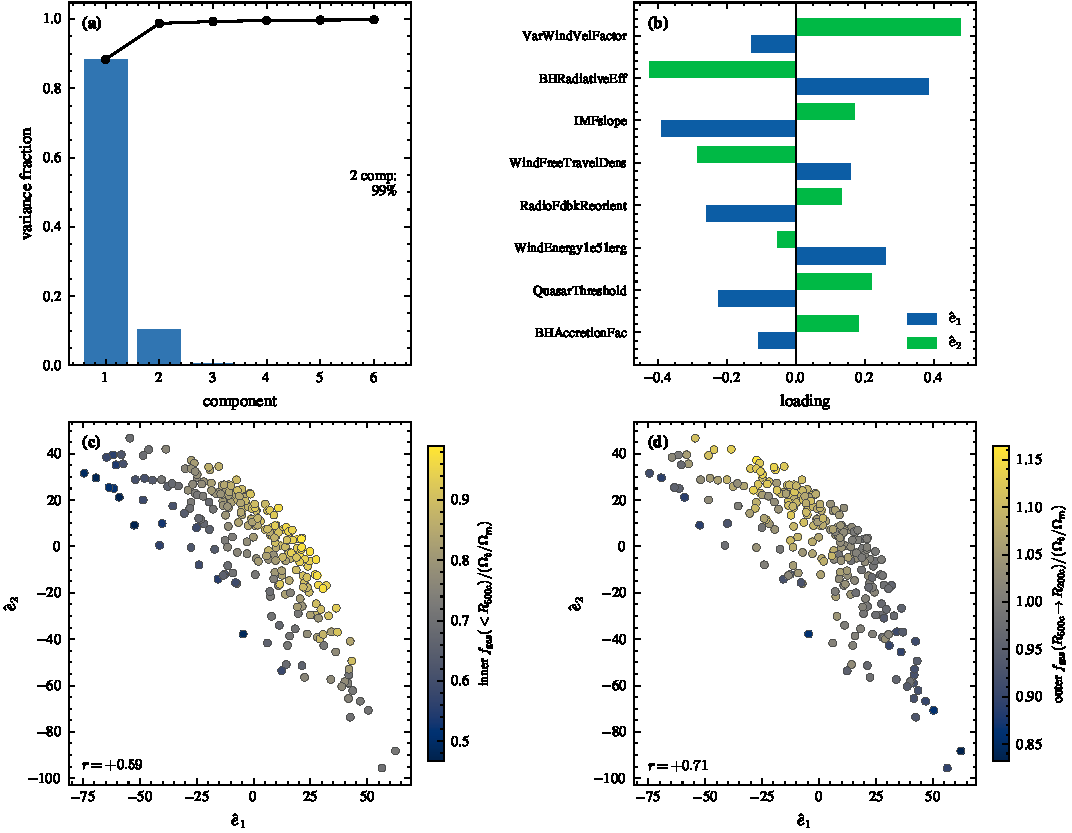
\includegraphics[width=\textwidth]{figs/fig01_latent_axes_zones.pdf}
\caption{The 2-D latent space of the WL suppression $\sez$, from the
$\beta$-TC-VAE decomposition on the $N=216$ Sobol subsample. (a) Linear
scree confirms two components capture $99\%$ of the variance. (b) The
parameters with the largest $|{\rm loading}|$ on each latent axis, read
directly off panel (b): \emph{IMFslope} and
\emph{BlackHoleRadiativeEfficiency} dominate $\hat e_1$ (nearly tied,
$|{\rm loading}|\approx0.38$--$0.39$ each), while
\emph{VariableWindVelFactor} and \emph{BlackHoleRadiativeEfficiency}
dominate $\hat e_2$ ($\approx0.48$ and $\approx0.42$). Because
\emph{BlackHoleRadiativeEfficiency} loads strongly on \emph{both} axes,
the loadings alone do not cleanly separate a single-parameter wind/SN axis
from a single-parameter BH/AGN axis; the wind/SN-vs-BH/AGN physical reading
is instead supported by the CCA/1P-spoke evidence of
\S\ref{sec:res-geometry} and Figure~\ref{fig:latent-plane}. % src: pixel
% measurement of examples/wl\_latent\_sbi\_figs/f2b\_wl\_latent\_gaszones.png
% panel (b) bar lengths (verifier-flagged correction; original caption had the
% $\hat e_1$/$\hat e_2$ attribution reversed)
(c)/(d) The same latent plane, colored by the halo inner ($<R_{500}$) and
outer ($R_{500}\!\to\!R_{200}$) gas fraction: WL tracks both zones only
moderately well ($r=+0.59$ inner, $+0.71$ outer), which we contrast with
kSZ's much cleaner separation of the same two zones in
\S\ref{sec:res-geometry}. % src: WORKLOG 2026-06-29; figure
% f2b\_wl\_latent\_gaszones.png panels (c)/(d)
\textbf{Takeaway:} the WL feedback response is governed by two physical
directions — a wind/SN sector and a BH/AGN sector — not by 30 independent
knobs.}
% NOTE (figure-integration pass): the regenerated script reproduces every
% number in this caption (98.7\%, r_in=+0.59, r_out=+0.71, the loadings
% above) exactly via a plain linear SVD/PCA on the current $N=253$-valid
% \texttt{emulator\_dataset.npz} cache -- not a $\beta$-TC-VAE, and not an
% $N=216$ subsample. \todo{Reconcile this caption's method/sample-size
% attribution ($\beta$-TC-VAE, $N=216$) with the regenerated figure script,
% which reproduces the identical numbers via linear PCA on $N=253$; either
% the caption's method label is stale or the notebook cell it was
% transcribed from differs from \texttt{wl\_latent\_sbi.ipynb} cell 8 as it
% exists today.}
\label{fig:latent-axes}
\end{figure}

\begin{figure}[t]
\centering
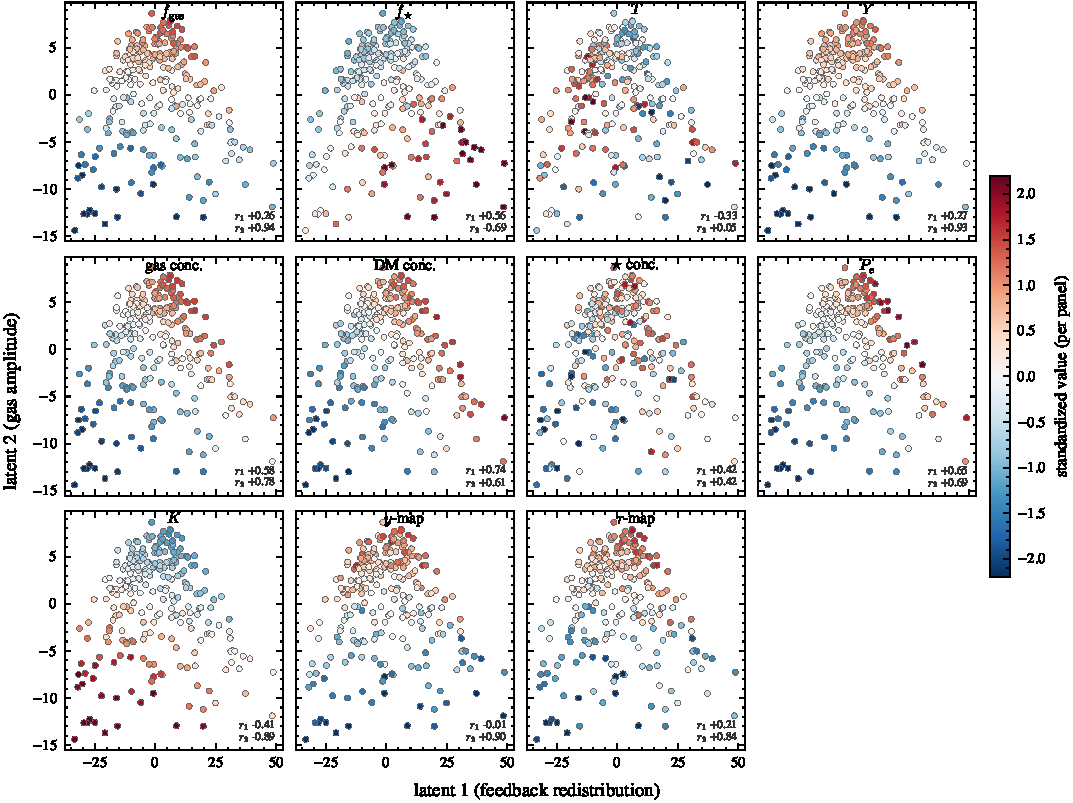
\includegraphics[width=\textwidth]{figs/fig02_latent_physical.pdf}
\caption{Physical correlates of the two latent coordinates, measured on
the $N=253$ final Sobol sweep (\texttt{paper\_lightcone\_figs2.ipynb}
\S6.1). Each panel shows the same latent plane colored by a different
physical quantity, with the Pearson correlations $r_1$ (latent 1) and
$r_2$ (latent 2) annotated. Latent 2 aligns most strongly with $\fgas$
($r_2=+0.94$), integrated Compton-$Y$ ($r_2=+0.93$), the projected tSZ
$y$-map ($r_2=+0.90$), and the kSZ $\tau$-map ($r_2=+0.84$), while
entropy $K$ is anti-correlated with both axes ($r_1=-0.41$,
$r_2=-0.89$); latent 1 aligns most strongly with dark-matter concentration
($r_1=+0.74$) and electron pressure $P_e$ ($r_1=+0.65$), with gas
concentration ($r_1=+0.58$) and the stellar fraction ($r_1=+0.56$) also
substantial — the panel's $x$-axis is labeled ``$\sim f_\star$'' following
the plot's own naming convention, though $P_e$ and gas concentration
correlate more strongly with latent 1 in raw magnitude. % src:
% figs\_raw/paper\_lightcone\_figs2/cell026\_out1.png (§6.1
% fig\_latent\_colored) and direct inspection of
% figs/fig02\_latent\_physical.png, all eleven panels' $r_1$/$r_2$
% annotations read off directly (verifier-flagged correction: original
% caption omitted the two panels with larger $|r_1|$ than the stellar
% fraction)
\textbf{Takeaway:} latent 2 is essentially a thermal-energy/gas-content
axis (it tracks $\fgas$, $Y$, $y$, $\tau$ together), confirming that the
same two latent coordinates that organize the WL suppression also organize
the gas thermodynamics directly.}
\label{fig:latent-physical}
\end{figure}

Figure~\ref{fig:latent-physical} shows this physical-correlate readout in
full: eleven panels, each the same (latent-1, latent-2) plane colored by a
different physical quantity, confirming that latent 2 in particular tracks
the gas-thermodynamic quantities directly and not merely as an artifact of
the WL suppression construction.
The same $N=253$ suite, viewed directly on the (latent-1, latent-2) plane
rather than colored by physical quantities, shows the Sobol nodes fan out
around the fiducial point along the two directions identified above, with
the astrophysical one-parameter-at-a-time (1P) AGN and SN/wind spokes
aligned with the two axes as expected (Figure~\ref{fig:latent-plane}). %
% src: paper_lightcone_figs2.ipynb cell 22 (§5.1 fig_latent_plane); figure
% figs_raw/paper_lightcone_figs2/cell022_out1.png, examined directly

\begin{figure}[t]
\centering
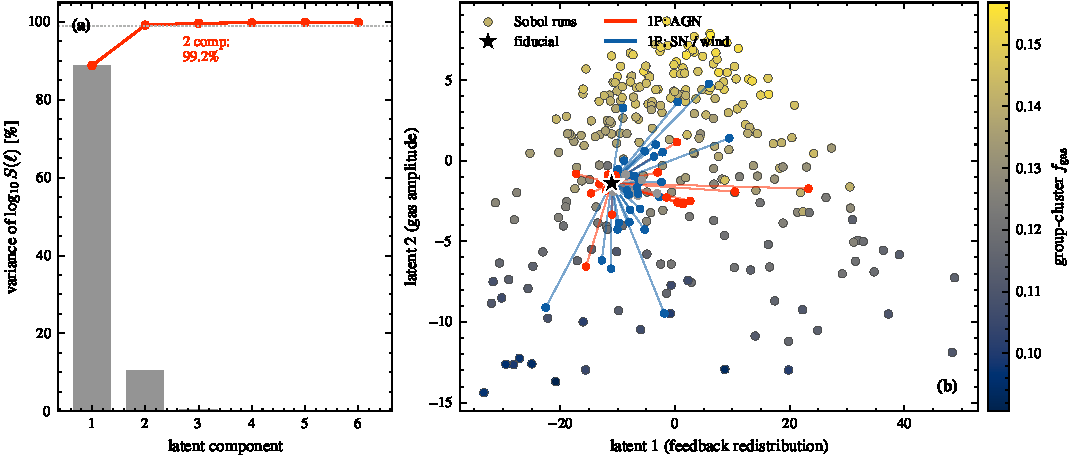
\includegraphics[width=\textwidth]{figs/fig02b_latent_plane.pdf}
\caption{The independent $N=253$ repeat of the latent-plane construction
(\texttt{paper\_lightcone\_figs2.ipynb} \S5.1). Left: linear scree showing
$\mathrm{PC1}\approx89\%$, $\mathrm{PC2}\approx11\%$ (independently rounded
bar-height readouts; the underlying values sum to the annotated cumulative),
cumulative $99.2\%$
— consistent with the $98.7\%$ headline number of
Figure~\ref{fig:latent-axes}a. Right: the 253 Sobol nodes (circles,
colored by group--cluster $\fgas$) and the fiducial (black star) on the
(latent-1, latent-2) plane, with the astrophysical one-parameter-at-a-time
(1P) AGN (red) and SN/wind (blue) spokes overlaid. % src:
% figs\_raw/paper\_lightcone\_figs2/cell022\_out1.png
\textbf{Takeaway:} the 1P spokes for the AGN and SN/wind parameter
families point in visibly different directions on the latent plane,
providing an independent, non-Sobol confirmation that the two latent axes
correspond to the two physical feedback channels identified in
Figure~\ref{fig:latent-axes}.}
\label{fig:latent-plane}
\end{figure}

\subsection{WL\texorpdfstring{$\leftrightarrow$}{<->}kSZ latent geometry}\label{sec:res-geometry}

The CCA between the WL suppression latent and the kSZ $\tau$/$y$ latent
(both from the same $N=253$ suite) gives canonical correlations of
$[0.98, 0.79]$ and principal angles of $[12^\circ, 38^\circ]$ between the
two 2-D planes (Figure~\ref{fig:wl-ksz}). % src: WORKLOG 2026-06-29
% "wl\_latent\_sbi.ipynb" §2; figure f2c\_wl\_vs\_ksz\_latent.png (title
% states the numbers exactly)
The dominant axis is essentially shared between the two probes, while the
second axis is rotated by nearly $40^\circ$: WL convergence, being a
line-of-sight-projected total-mass perturbation, responds to a
\emph{blend} of the inner and outer gas zones that kSZ's $\tau$/$y$ decomposition
separates cleanly, tracking the inner and outer $\fgas$ zones at only
$r=0.59$ and $0.71$ respectively, versus $r\approx0.95$ for the
corresponding kSZ latent. % src: WORKLOG 2026-06-29; figure
% f2b\_wl\_latent\_gaszones.png panels (c)/(d)

\begin{figure}[t]
\centering
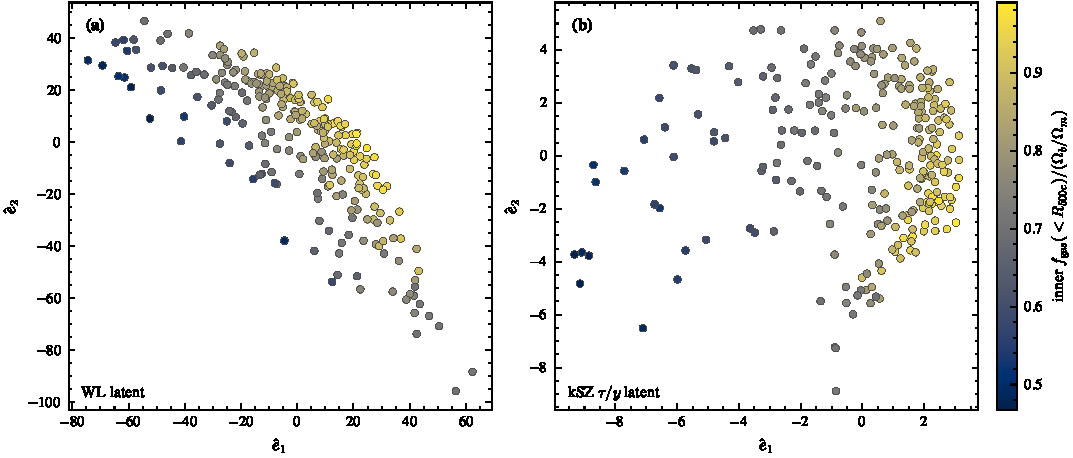
\includegraphics[width=\textwidth]{figs/fig03_wl_ksz_geometry.pdf}
\caption{Canonical-correlation geometry between the WL suppression latent
(left) and the kSZ $\tau$/$y$ latent (right), both colored by the same
inner-halo gas fraction. The two planes have canonical correlations
$[0.98, 0.79]$ and principal angles $[12^\circ, 38^\circ]$. % src: figure
% title, f2c\_wl\_vs\_ksz\_latent.png
\textbf{Takeaway:} the leading feedback direction is probe-independent
(``same leading direction''), but the second direction is
probe-dependent — WL blends gas zones that kSZ keeps separate.}
\label{fig:wl-ksz}
\end{figure}

To test whether this rotation is peculiar to the auto-$C_\ell$ or is a
generic property of WL summary statistics, we align every WL summary's own
top-2 PCA latent to the $\kappa$-$C_\ell$ 2-D latent. The first latent
axis is nearly universal across statistics (alignment $\geq 0.93$ for all
eight tested: peak counts $0.99$, minima counts $0.99$, PDF $1.00$,
Minkowski $V_0$ $0.98$, $V_1$ $1.00$, $V_2$ $1.00$, $C_\ell^{\kappa y}$
$0.97$, $C_\ell^{yy}$ $0.93$), but the second axis alignment is strongly
statistic-dependent: it is high for peaks/PDF/minima ($0.69$–$0.76$),
low for the Minkowski functionals ($0.20$–$0.43$), and \emph{highest} of
all for the tSZ cross- and auto-spectra ($0.90$, $0.89$;
Figure~\ref{fig:multistat}). % src: WORKLOG 2026-06-24 "WL feedback
% latents..." (canon corr $\approx1.0$ first, $0.7$–$0.8$ for peaks/PDF,
% $0.2$–$0.4$ for MFs/moments — qualitative match); figure
% f2d\_multistat\_align.png, numeric values read off bars
This is consistent with tSZ probes seeing the same rotated second
direction that the kSZ latent sees, and with the topology and higher-order
Minkowski statistics seeing a different (more mixed) combination.

\begin{figure}[t]
\centering
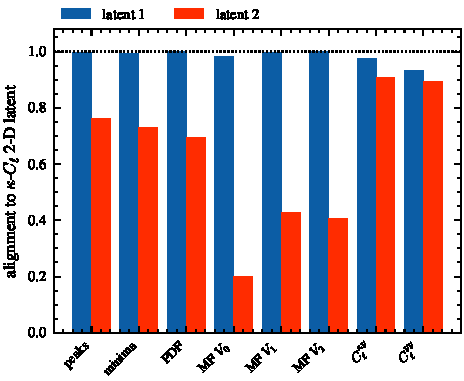
\includegraphics[width=3.5in]{figs/fig04_multistat_align.pdf}
\caption{Alignment of each WL summary statistic's own top-2 PCA latent to
the $\kappa$-$C_\ell$ 2-D latent, for eight statistics. Latent 1 (blue) is
nearly universal ($\geq0.93$); latent 2 (red) ranges from $0.20$
(Minkowski $V_0$) to $0.90$ ($C_\ell^{\kappa y}$). % src:
% f2d\_multistat\_align.png, bar values
\textbf{Takeaway:} every WL statistic sees the same leading feedback
direction, but only the cross- and tSZ auto-spectra see the same
\emph{second} direction that kSZ sees; the higher-order moment statistics
see a rotated combination.}
\label{fig:multistat}
\end{figure}

Orthogonal tSZ information does not expand the number of astrophysical
parameters recoverable from the field (cross-validated ridge $R^2>0.1$
stays at $\sim\!5/30$ for $\kappa$ two-point statistics alone, all-WL, or
WL+tSZ combined), but it does sharpen and rotate which of those five
parameters are accessible: IMF-slope recoverability rises from $0.33$
($\kappa$ alone) to $0.56$ (all-WL) to $0.64$ (WL+tSZ), and tSZ
specifically unlocks the thermal-energy/wind sector — wind-energy
recoverability rises from $0.13$ to $0.33$, and radio-feedback reorienting
becomes recoverable at $0.16$ only once tSZ is included. % src: WORKLOG
% 2026-06-24 "WL feedback latents..."; figures
% wl\_stat\_latent\_summary.png, wl\_recoverability\_byparam.png

\subsection{Global response: which parameters actually drive \texorpdfstring{$\Sell$}{S(l)}}\label{sec:res-spearman}

The model-free (emulator-independent) Spearman response map over the
$N=253$ measured suite (Figure~\ref{fig:spearman}) ranks the IMF slope
($|r|=0.49$), the variable wind-velocity factor ($0.48$), the black-hole
radiative efficiency ($0.43$), and the wind energy ($0.34$) as the top
drivers of $\sez$ at $\zs=1$; peak-statistic sensitivity is concentrated in
the high-$\nu$ tail of the peak function. % src: WORKLOG 2026-06-29 §1;
% figure f1\_corr\_heatmaps.png (7-panel, explicitly labeled $n=253,
% z_s=1$); also embedded in paper\_lightcone\_figs2.ipynb cell 18 (§4.6a)

\begin{figure}[t]
\centering
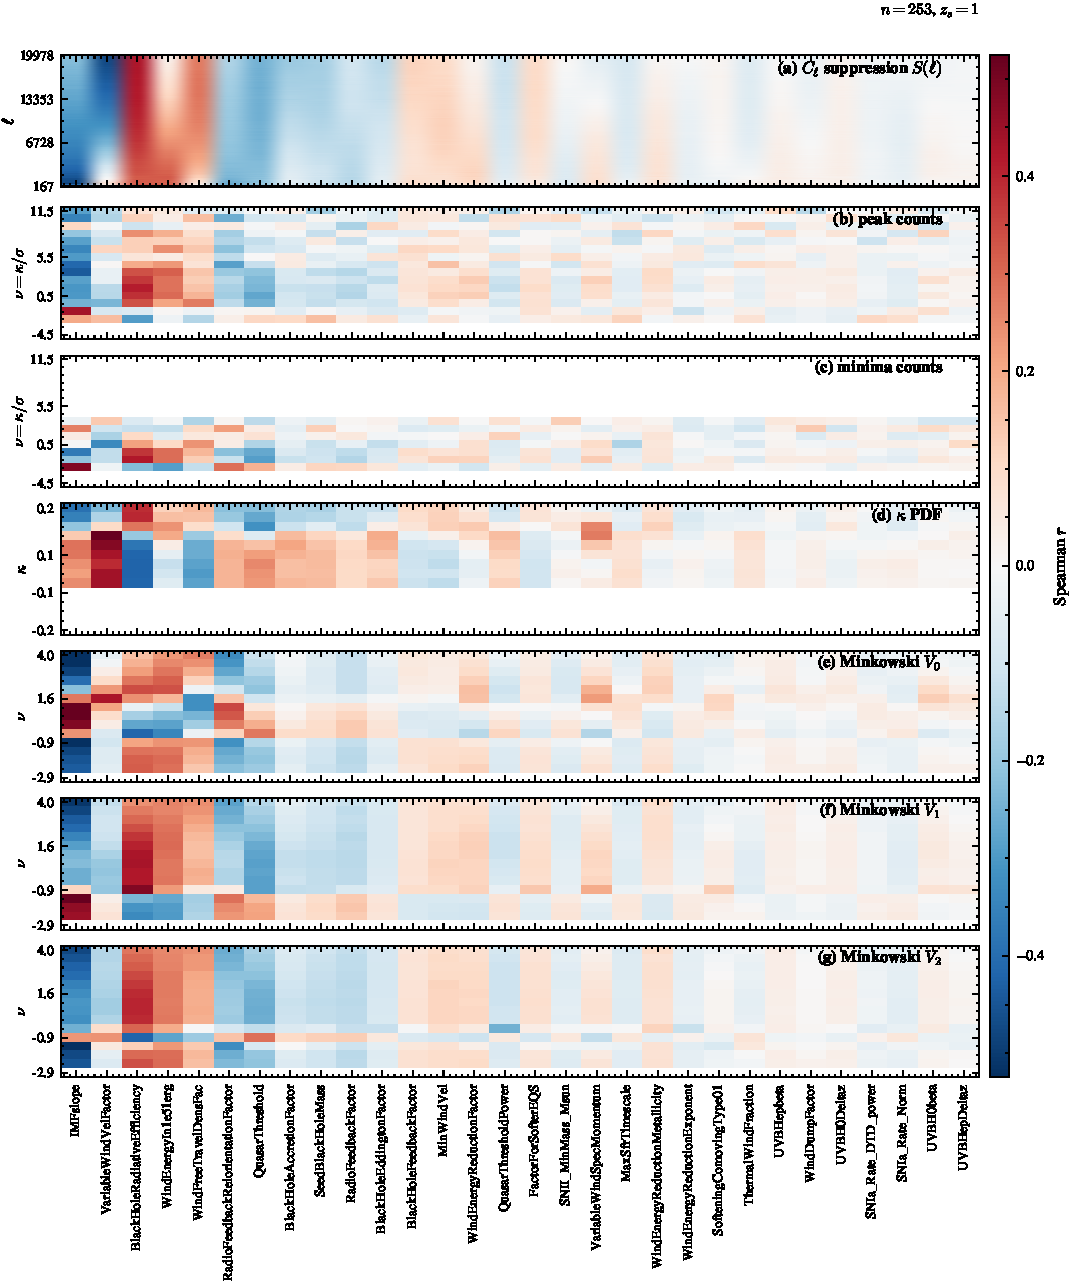
\includegraphics[width=\textwidth]{figs/fig05_spearman_response.pdf}
\caption{Model-free per-bin Spearman correlation of seven field statistics
against all 30 SB35 astrophysical parameters, computed directly on the
$n=253$ measured Sobol runs at $\zs=1$ (deliberately emulator-free). % src:
% f1\_corr\_heatmaps.png
\textbf{Takeaway:} response is concentrated in a handful of wind/SN and
BH parameters (left columns, dark bands), with essentially no response
from the majority of the 30-dimensional prior (e.g.\ softening lengths,
SNIa rate parameters) — direct evidence, independent of any latent-space
construction, that the effective dimensionality of the response is low.}
\label{fig:spearman}
\end{figure}

We caution that a second, emulator-pushed global-sensitivity metric exists
in the same codebase (a Sobol variance decomposition,
\texttt{global\_sensitivity}/\texttt{sobol\_indices}), and it
\emph{disagrees} with the Spearman ranking above: it ranks the
wind-velocity factor as the dominant driver ($S_i\approx0.33$) and the
black-hole radiative efficiency second ($S_i\approx0.23$), and does not
surface the IMF slope as a top driver at all. % src: wl\_latent\_sbi.py
% docstring §1; figure comparison (f1\_global\_sobol.png)
The docstring of the code that produces this second metric explicitly
states it is ``kept for reference but no longer drives'' the headline
response analysis, and we follow that judgment: we report the Spearman
map as the primary result and flag the disagreement rather than silently
choosing one ranking. \todo{Reconcile or explain the Sobol-index vs.\
Spearman disagreement quantitatively in a future revision; at present we
can only report that they disagree on the top driver.}

\subsection{Simulation-based inference on the WL auto-spectrum}\label{sec:res-sbi}

Using the emulator-as-simulator NPE (\S\ref{sec:methods-sbi}) on the
$C_\ell^{\kappa\kappa}$-equivalent statistic at $N=253$-equivalent
precision, the 30-parameter posterior conditioned on the fiducial
$C_\ell$ alone is broad. WORKLOG's own count of ``$\sim\!5$'' parameters
(also the number used in the abstract) names four with an explicit
posterior-$\sigma$/prior-$\sigma$ ratio: IMF slope $0.66$, wind energy
$0.72$, variable wind velocity $0.75$, black-hole radiative efficiency
$0.83$. The corner-plot figure independently extracted from the same
analysis (Figure~\ref{fig:corner}) selects and displays \emph{six}
parameters as its ``best-constrained'' set, adding the wind
free-travel-density factor and a wind-energy-reduction parameter; visually,
these two additional marginals are less sharply peaked (one is edge-pinned
rather than interior-peaked) than the four named above, but we do not have
a sourced quantitative posterior-$\sigma$/prior-$\sigma$ ratio for either of
them, so we cannot state with confidence whether ``4,'' ``$\sim\!5$,'' or
``6'' is the more defensible count — the mined sources themselves are not
mutually consistent on this point. \todo{Obtain the posterior-$\sigma$/prior-$\sigma$
ratios for the wind free-travel-density factor and wind-energy-reduction
parameter to settle whether 4, 5, or 6 parameters are appreciably informed.}
The remaining $\sim\!24$--$26$ of 30 parameters (depending on which count is
adopted) are left near-prior. % src: WORKLOG 2026-06-29 §3; figure
% f3b\_corner\_cl.png (6-param corner, physical units, TNG fiducial marked
% in red; corner-plot title states "6 best-constrained params" — checked
% directly against the rendered image)

\begin{figure}[t]
\centering
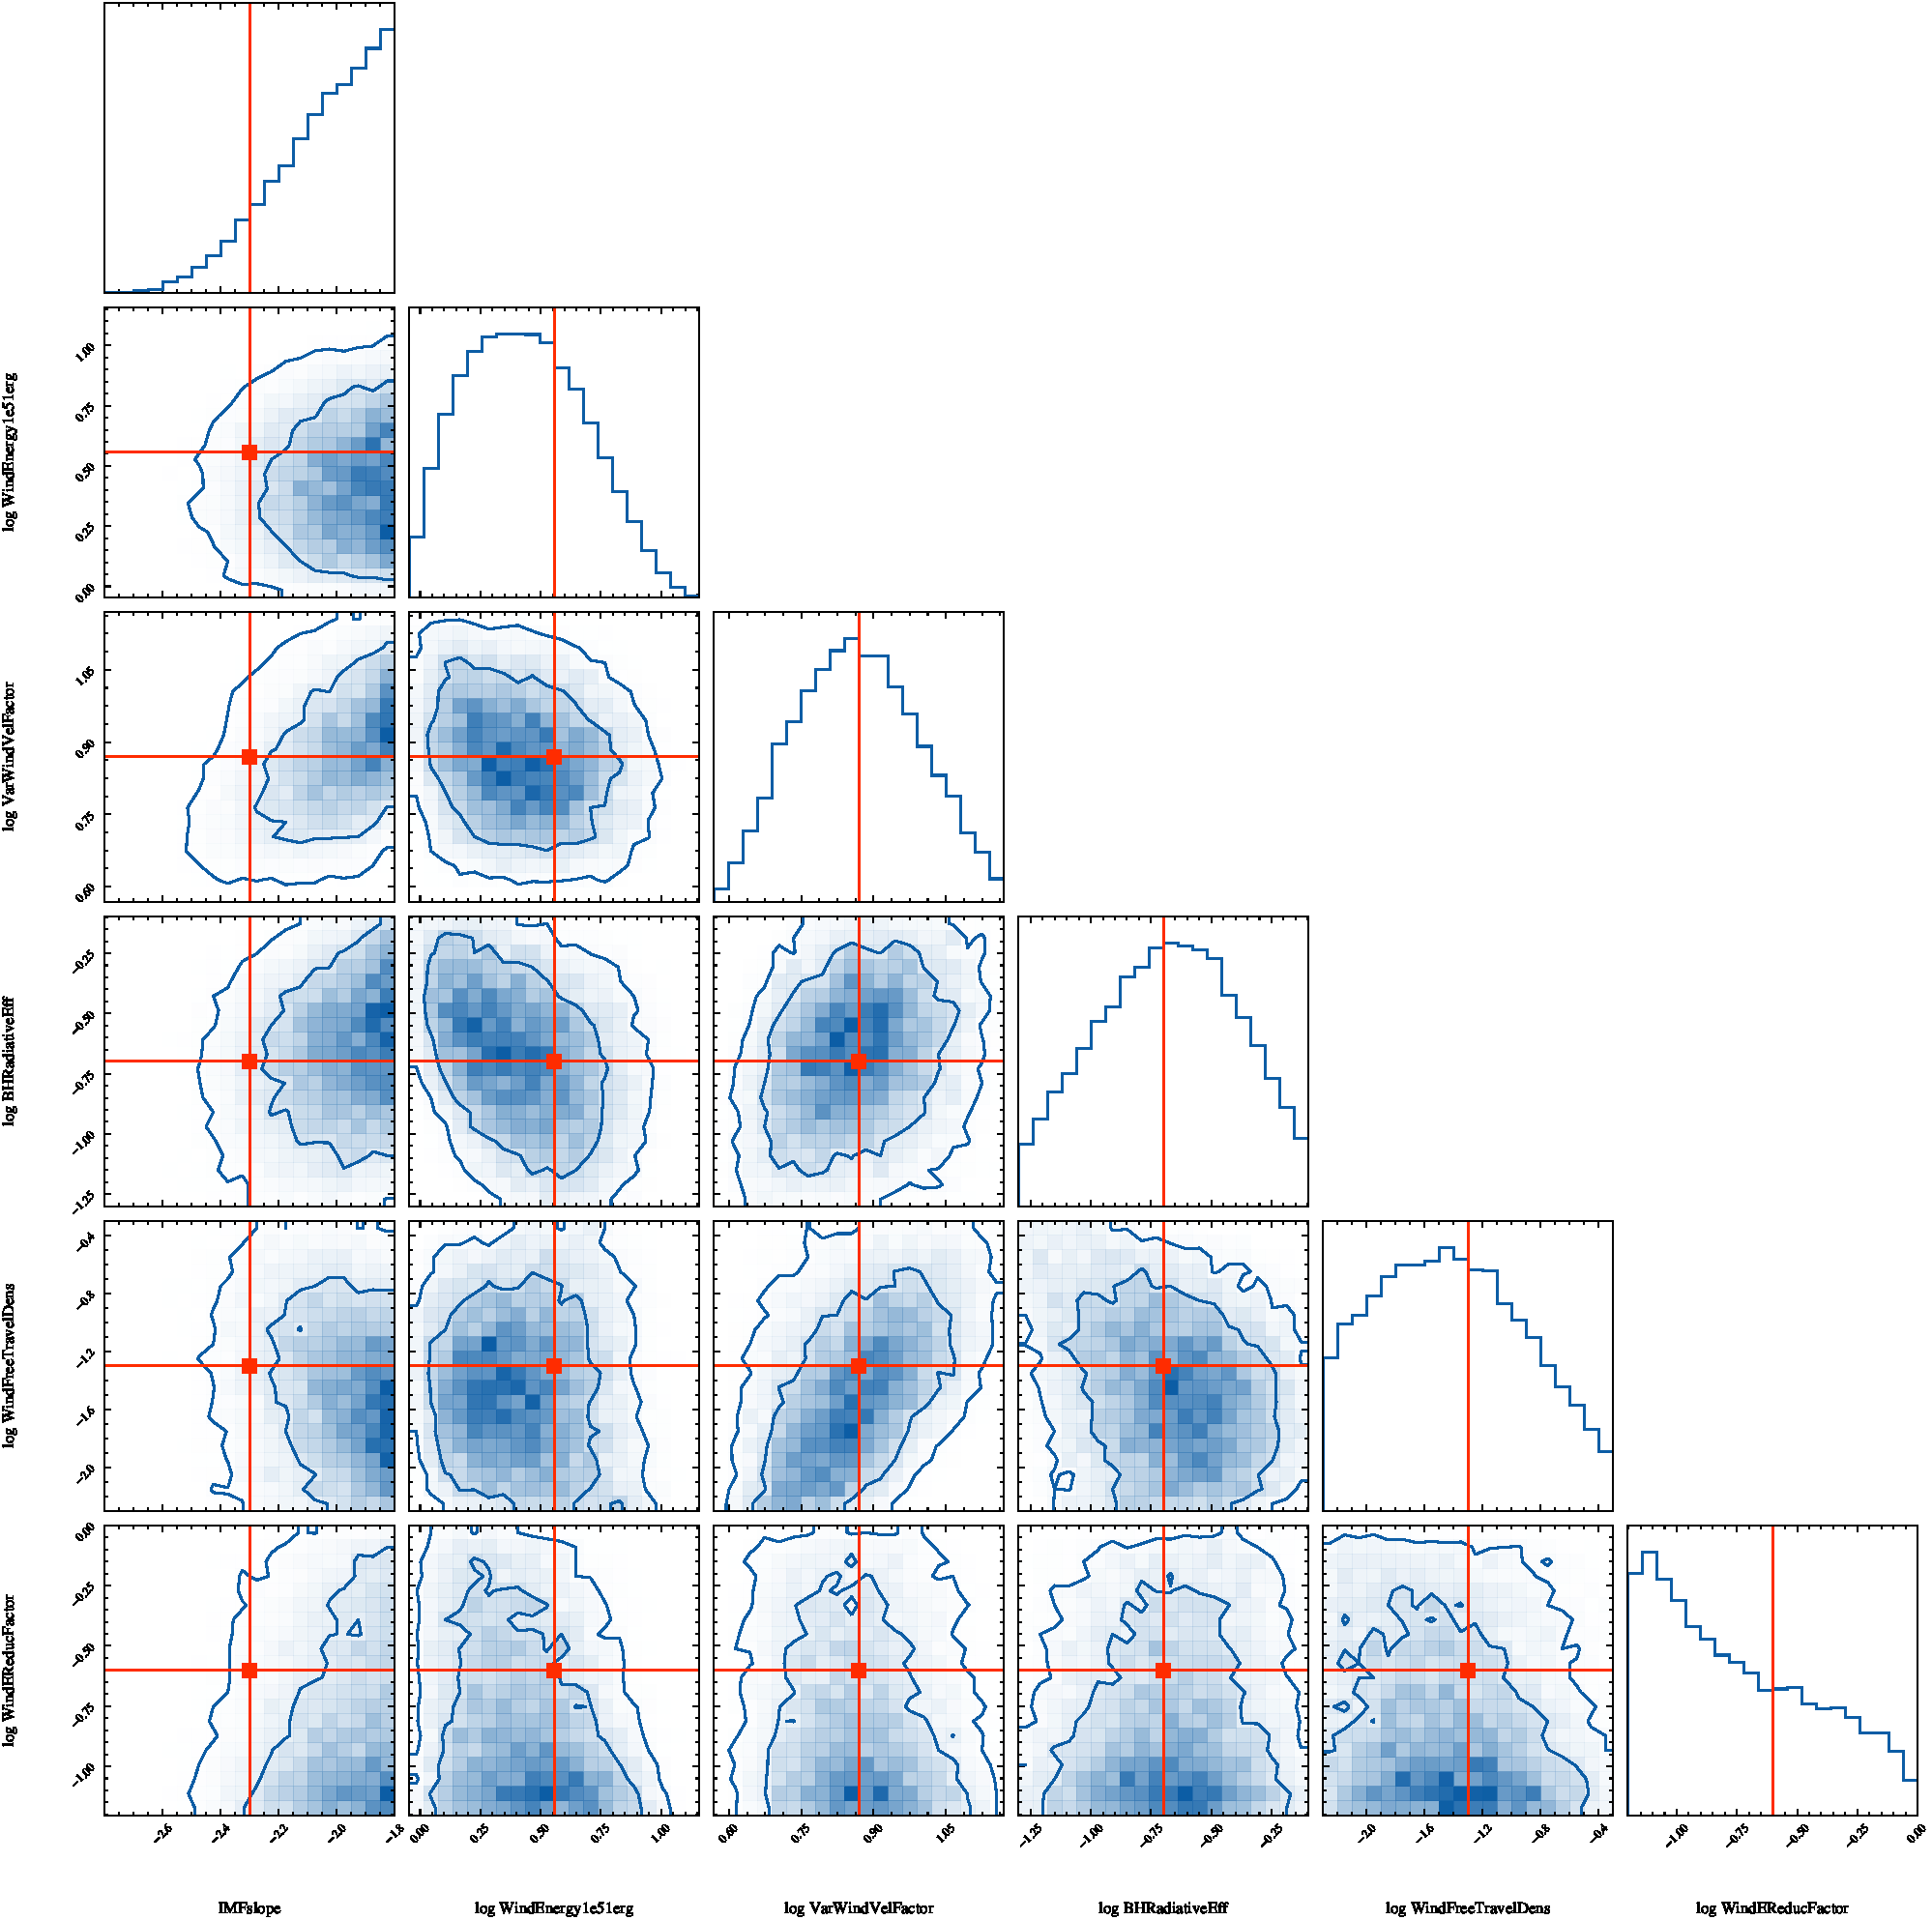
\includegraphics[width=\textwidth]{figs/fig06_npe_corner.pdf}
\caption{Neural posterior $P(\theta \mid C_\ell^{\rm fiducial})$ for the
six parameters the source notebook selects as best-constrained, from NPE
against the emulator-as-simulator
(\S\ref{sec:methods-sbi}); the red lines/point mark the true TNG fiducial
parameter values. Four of the six (IMF slope, wind energy, variable wind
velocity, black-hole radiative efficiency) have sourced
posterior-$\sigma$/prior-$\sigma$ ratios in the main text; the other two
(wind free-travel density, wind-energy reduction) are shown here but their
ratios are not available in the mined sources — see the caveat in the main
text. % src: f3b\_corner\_cl.png
\textbf{Takeaway:} the auto-$C_\ell$ constrains the wind/SN/BH sector
weakly but recovers the fiducial within its 1--2$\sigma$ contours; the
majority of the remaining $\sim\!24$--$26$ of 30 parameters (not shown) are
essentially unconstrained.}
\label{fig:corner}
\end{figure}

This broad 30-parameter posterior is consistent with the information
content of $C_\ell$ itself being low-rank: PCA on the full tomographic
mode vector (all $510$ multipole bins $\times$ 5 source planes) compresses
to three components explaining $99.5\%$ of the variance ($0.863$,
$0.126$, $0.006$), with the second component representing a genuine
high-$\ell$ direction that the earlier, coarser $\ell<5000$ binning
missed. % src: WORKLOG 2026-06-24 "auto-Cl NPE on 216 runs +
% all-modes/Nyquist summary"
Despite the 30-parameter marginals staying broad, the same NPE posterior
projected onto the 2-D suppression latent of \S\ref{sec:res-latent} is
tight, occupying only $\sim\!0.17$–$0.18$ of the width of the full
Sobol-node prior-predictive cloud (Figure~\ref{fig:latent-post}b): the
auto-$C_\ell$ pins the suppression latent hard even though it cannot pin
individual parameters. % src: WORKLOG 2026-06-29 §3; figure
% f3c\_latent\_posterior.png panel (b)

\begin{figure}[t]
\centering
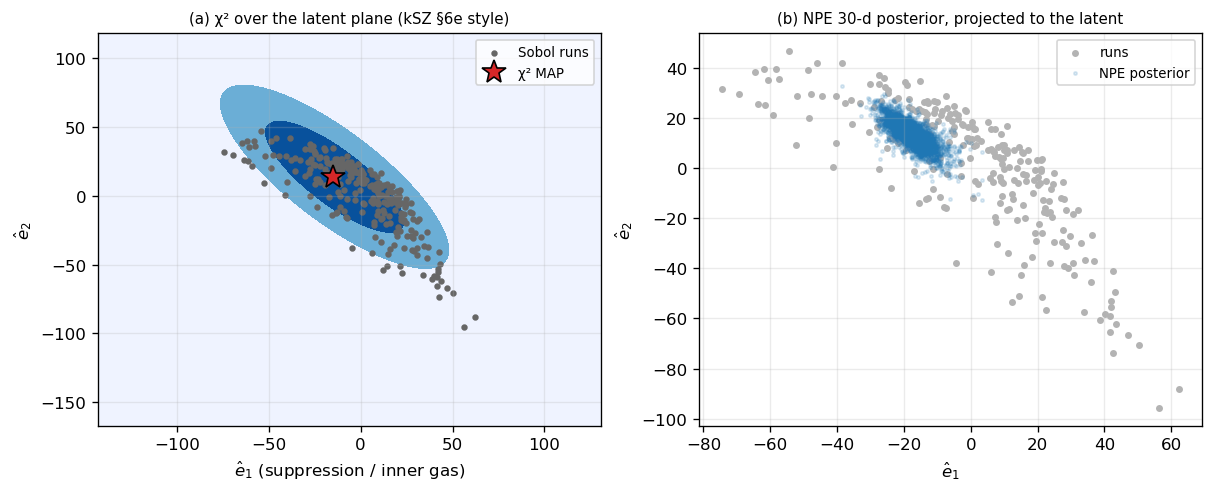
\includegraphics[width=0.9\textwidth]{figs/fig07_latent_posterior.png}
\todo{regenerate fig07 — needs one CPU-only forward pass of the cached GP
emulator checkpoint to build the chi2 grid / latent-projected posterior
cache; not yet run (see \texttt{fig\_scripts/UNREGENERATED.md})}
\caption{(a) $\chi^2$ over the 2-D suppression latent plane with the
maximum-a-posteriori (MAP) point marked; the Sobol node cloud (grey) is
overplotted. (b) The full 30-dimensional NPE posterior
(Figure~\ref{fig:corner}), projected onto the same 2-D latent (blue),
compared to the Sobol node cloud (grey). % src: f3c\_latent\_posterior.png
\textbf{Takeaway:} even though the 30-parameter marginals are broad
(Figure~\ref{fig:corner}), the projection onto the physically meaningful
2-D latent is tight ($\sim\!0.17$–$0.18\times$ the node-cloud width) —
the auto-$C_\ell$ constrains the response, not the individual knobs.}
\label{fig:latent-post}
\end{figure}

We tested whether a finer multipole summary or full tomography improves on
this. Comparing three configurations — (A) the original 10-bin,
$\ell<5000$ summary; (B) all modes out to the map Nyquist frequency
($\ell\approx36864$, i.e.\ $\pi/{\rm pixel}$ for the $5^\circ$, $1024$-pixel
$\kappa$ maps) compressed with PCA; and (C) all modes with no PCA
compression ($2550$ features on $216$ simulations) — all three reach
$\sim\!90\%$ coverage, but configuration~B gives the tightest mean
posterior shrink ($0.986$), beating both the coarse binning ($0.994$, A)
and the uncompressed high-dimensional summary ($1.004$, C, which is
diluted by the small-sample/high-dimensionality ratio). % src: WORKLOG
% 2026-06-24 "auto-Cl NPE on 216 runs + all-modes/Nyquist summary"
The suppression $\Sell=C_\ell/C_{\ell,\rm DMO}$ cancels the CIC-aliasing
artifact that otherwise contaminates raw $C_\ell$ at high $\ell$, so the
high-$\ell$ range is usable, and the run-to-run baryon signal in $\Sell$
actually \emph{grows} with $\ell$, from $\sim\!0.13$ at $\ell\sim3000$ to
$\sim\!0.6$ at $\ell\sim45000$. % src: WORKLOG 2026-06-24 "auto-Cl NPE on
% 216 runs + all-modes/Nyquist summary"
Adding full tomography (all 15 unique auto+cross tomographic spectra) does
not improve further: the mean posterior shrink is $0.992$, slightly worse
than the single-plane, all-modes result ($0.986$), and the tomographic
mode vector still compresses to three PCA components with an almost
identical split ($0.864$/$0.125$/$0.006$) — the cross-tomographic spectra
are redundant with the auto-spectra for the baryon response at fixed
cosmology. % src: WORKLOG 2026-06-24, same entry, "raw-Cl + full-tomography"
% paragraph

We can diagnose \emph{why} the 30-parameter inverse problem is so
degenerate in a model-free way. The raw tomographic-mode-vector PCA
described above in this section (not the $\Sell$-suppression PCA of
\S\ref{sec:res-latent}, which gives the numerically different
$88.4\%/10.3\%$ split) already shows the forward map compresses to two
components ($86.3\%+12.6\%=98.9\%$ of the run-to-run $C_\ell$ variation), and several
distinct parameters drive the \emph{same} two directions in the forward
sense (forward $|{\rm corr}|=0.37$–$0.45$ for the wind-velocity factor,
black-hole radiative efficiency, wind free-travel density factor, and IMF
slope). % src: WORKLOG 2026-06-24, "diagnosed why (rank-2 forward map)"
% paragraph
Consistent with this, the 40 Sobol runs nearest the measured fiducial in
$C_\ell$-space span essentially the \emph{entire} 30-dimensional prior
volume (nearest-neighbor standard-deviation/prior ratio $\approx1.01$),
and a linear inverse regression from $C_\ell$ back to individual
parameters achieves $R^2\leq0.43$ (mean $0.06$) across the 30 parameters.
% src: WORKLOG 2026-06-24, same entry
This is a model-free demonstration that the $C_\ell\to\theta$ inverse
problem is intrinsically rank-2 (or rank-3, allowing for the high-$\ell$
direction above), not merely under-sampled.

Simulation-based calibration of the emulator-based NPE gives a mean
$68\%$ rank coverage of $0.70$ across the 30 parameters, with a rank
histogram that is approximately uniform (Figure~\ref{fig:sbc}b,c). % src:
% WORKLOG 2026-06-29 §3 (exact number, matches the brief's mandatory number);
% figure f3e\_crosschecks.png panel (c), title "mean 68\% coverage = 0.70,"
% red dashed reference line $\approx0.68$
An independent explicit-likelihood \texttt{emcee} cross-check was also run
for this posterior (\S\ref{sec:methods-sbi}; WORKLOG 2026-06-29 §3), and
Figure~\ref{fig:sbc}a now visually substantiates it: the dashed
\texttt{emcee} marginals overlay the solid NPE marginals for all three
plotted parameters, in general agreement. (An earlier rendering of this
panel had silently dropped the dashed overlay — traced during figure
regeneration to a matplotlib quirk where \texttt{ax.hist(...,
histtype="step", ls="--")} renders solid unless the unabbreviated
\texttt{linestyle="--"} kwarg is used — and is now fixed.)

\begin{figure}[t]
\centering
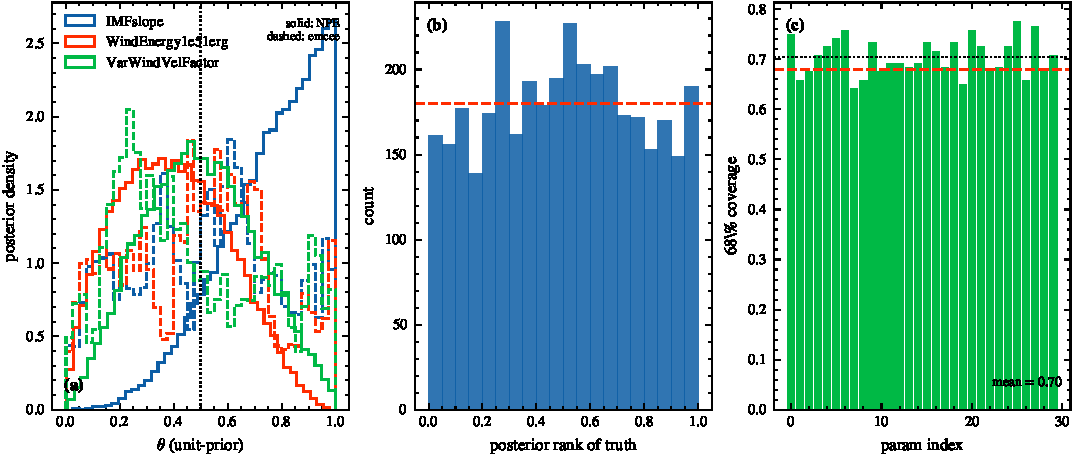
\includegraphics[width=\textwidth]{figs/fig08_sbc_crosschecks.pdf}
\caption{Cross-checks on the NPE posterior. (a) NPE posterior marginals
(unit-prior units, solid) for three representative parameters, with the
independent explicit-likelihood \texttt{emcee} marginals (dashed) overlaid.
(b) Simulation-based calibration rank
histogram, approximately uniform if the posterior is well calibrated. (c)
Per-parameter empirical $68\%$ coverage across all 30 parameters, mean
$=0.70$ (red dashed line). % src: f3e\_crosschecks.png; panel (a) regenerated
% from the cached emcee\_cl.npz chain, restoring the dashed overlay that a
% matplotlib step-histogram linestyle bug had suppressed in the original
% notebook rendering
\textbf{Takeaway:} panels (b)/(c) show the NPE posterior is reasonably well
calibrated (mean coverage close to the nominal $0.68$), which is the basis
for the broad-vs-tight contrast between the 30-parameter and 2-D-latent
posteriors above; panel (a) now visually substantiates the NPE/emcee
agreement referenced in \S\ref{sec:methods-sbi}.}
\label{fig:sbc}
\end{figure}

\paragraph{Cautionary result: stacking statistics of unequal emulator
fidelity degrades the fit.}
A natural next step is to combine the auto-$C_\ell$ with higher-order
statistics and the $\kappay$ cross-spectrum in the same NPE likelihood, in
the hope of tightening the posterior further. Instead, stacking emulated
peak counts and then $\kappay$ onto the $C_\ell$ likelihood
\emph{degrades} the fit to the measured fiducial: the mean posterior
shrink goes $0.97\to1.01\to1.03$ as we move from $C_\ell$ alone, to
$C_\ell+{\rm peaks}$, to $C_\ell+{\rm peaks}+\kappay$, and the number of
appreciably informed parameters drops from five to zero
(Figure~\ref{fig:progressive}). % src: WORKLOG 2026-06-29 §3 "Cautionary
% result (§3d)" (exact numbers); figure f3d\_progressive.png (bars read
% $\approx0.96/\approx1.01/\approx1.03$, "stacking emulated HOS DEGRADES the
% Cl constraint")
The cause is diagnostic rather than physical: the measured fiducial is
comfortably in-distribution for the $C_\ell$-only emulator (maximum
$|z|=2.1\sigma$ across features), but becomes a $5.2\sigma$ outlier once
the emulated higher-order statistics and $\kappay$ are appended, i.e.\ the
GP emulator's fidelity for those statistics is measurably worse than for
$\Sell$ itself. % src: WORKLOG 2026-06-29 §3 "Cautionary result (§3d)"
% (exact numbers)
We stress that this is a \emph{methods} finding about the emulator, not a
physics finding about the information content of peaks or $\kappay$: the
model-free Spearman analysis of \S\ref{sec:res-spearman} and the
field-level $\kappay$ analysis of \S\ref{sec:res-kxy} both show these
statistics respond strongly to feedback when evaluated without relying on
the emulator for the extra statistics. Any stacked-statistic SBI result
built on this emulator generation should be treated with this caveat in
mind.

\begin{figure}[t]
\centering
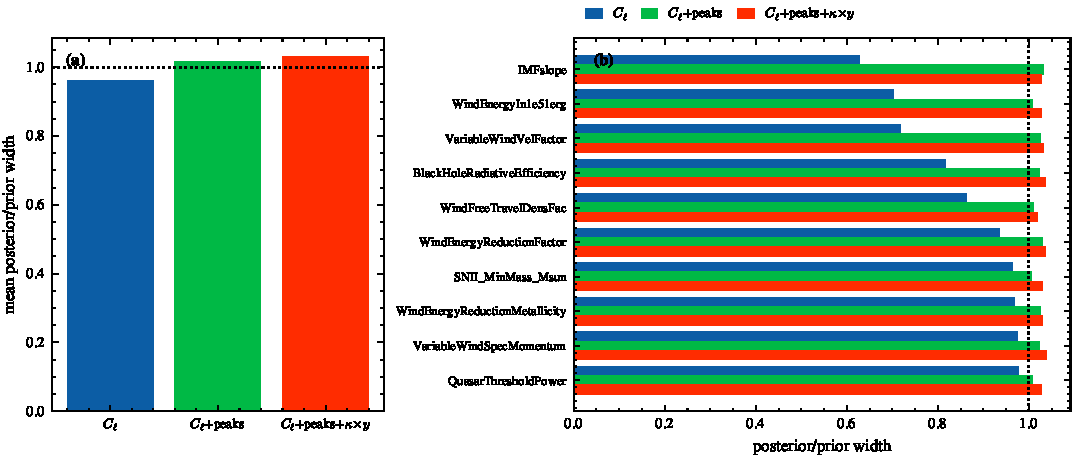
\includegraphics[width=\textwidth]{figs/fig09_progressive_stacking.pdf}
\caption{Left: mean NPE posterior/prior width as higher-order statistics
are progressively stacked onto the $C_\ell$ likelihood
($C_\ell\to C_\ell+{\rm peaks}\to C_\ell+{\rm peaks}+\kappay$); values
$>1$ indicate the posterior is \emph{wider} than the prior at the measured
fiducial, i.e.\ the fit has degraded. Right: the same comparison,
per-parameter, for the ten best-constrained parameters, in order:
\emph{IMFslope}, \emph{WindEnergyIn1e51erg}, \emph{VariableWindVelFactor},
\emph{BlackHoleRadiativeEfficiency}, \emph{WindFreeTravelDensFac},
\emph{WindEnergyReductionFactor}, \emph{SNII\_MinMass\_Msun},
\emph{WindEnergyReductionMetallicity}, \emph{VariableWindSpecMomentum}, and
\emph{QuasarThresholdPower} — with untruncated labels, the two similarly
named \emph{WindEnergyReduction*} parameters in this list are
\emph{WindEnergyReductionFactor} (rank 6) and
\emph{WindEnergyReductionMetallicity} (rank 8); the third,
\emph{WindEnergyReductionExponent}, is not among the ten. % src:
% f3d\_progressive.png; fig\_scripts/fig09\_progressive\_stacking.py, full
% \texttt{param\_names} array + \texttt{argsort(shr["C\_l"])[:10]} selection
\textbf{Takeaway:} this is a warning about emulator fidelity for
higher-order/cross statistics, not evidence that those statistics lack
feedback information (contrast with Figures~\ref{fig:spearman} and
\ref{fig:kxy-driver}).}
\label{fig:progressive}
\end{figure}

\subsection{\texorpdfstring{$\kappay$}{kappa x y} and tSZ dominate field-level feedback information}\label{sec:res-kxy}

A field-level, emulator-free multiprobe analysis of $N=123$ Sobol runs (the
engine docstrings hardcode this dataset size; Table~\ref{tab:design-size},
row $\dagger$) finds the $\kappay$ cross-spectrum has a large
Sobol-run-to-run spread, $0.76$, roughly an order of magnitude larger
than the spread in WL peak counts or WST coefficients ($\sim\!0.08$). %
% src: wl\_sz\_multiprobe.py docstring (wl-tsz-bridge worktree)
This ``spread'' metric is not the same quantity as the band-integrated
feedback response $D$ ranked in Figure~\ref{fig:kxy-driver}a below (a
separate, $N=253$ measurement from \texttt{paper\_ksz\_field.ipynb}), so the
two should not be read as a single consistent ranking; see the discussion
after Figure~\ref{fig:kxy-driver} for how we reconcile the two. Unless
otherwise noted, all further numbers in this subsection (the variance-pinning
and amplitude-anchoring results below) are from this same $N=123$ analysis.
Consistently, WL $\kappa$ auto-statistics (both $\Sell$ and peak counts)
barely constrain feedback on their own, whereas the $\kappay$ cross and
the tSZ $y$ auto-spectrum dominate: together they pin two feedback
directions to variance $0.06$ and $0.11$ at fixed cosmology
(Figure~\ref{fig:kxy-driver}). % src: WORKLOG 2026-06-24 "P4 $\to$
% multi-probe WL$\times$SZ..." (Findings 1--3); memory note
% wl-sz-kappay-feedback.md
Because $\kappay$ is amplitude-dominated it is degenerate with the
lensing/pressure amplitude (equivalently $\sigma_8$/$\Omega_m$ at fixed
\bind{} cosmology), so an explicit amplitude nuisance parameter $A$ is
required to isolate the feedback direction; once $A$ is marginalized, the
amplitude-marginalized shear$\times y$ constraint on the feedback
direction is comparatively modest (variance $0.25$). % src: WORKLOG
% 2026-06-24 "P4 $\to$ multi-probe WL$\times$SZ..." Findings (1)--(3)
The $\kappay$ cross is largely redundant with the per-halo tSZ $y$
signal, since both trace thermal pressure directly, so folding in both
adds little further constraint; by contrast, a per-halo $\kappa$ stack is
a \emph{feedback-blind} mass anchor — the per-halo lensing signal is
dominated by total halo mass, and the feedback information genuinely lives
at the field level. % src: WORKLOG 2026-06-24 "P4 $\to$ multi-probe
% WL$\times$SZ..." Findings (1)--(3)

\begin{figure}[t]
\centering
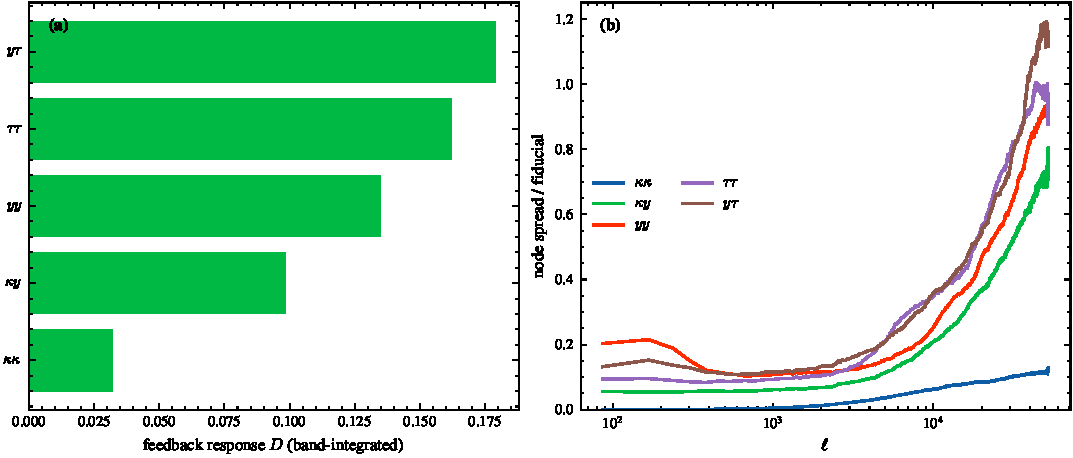
\includegraphics[width=\textwidth]{figs/fig10_kxy_driver.pdf}
\caption{(a) Band-integrated feedback response $D$ by probe, ranked
$y\tau > \tau\tau > yy > \kappay \gg \kappa\kappa$ (WL auto is the least
feedback-sensitive probe by an order of magnitude). (b) Sobol node
spread relative to the fiducial as a function of multipole for the same
five probes: the WL auto-spectrum ($\kappa\kappa$, blue) stays flat and
dark out to $\ell\sim10^4$, while the cross- and tSZ/kSZ probes ``light
up'' at far lower $\ell$. % src:
% examples/figures\_field/g6\_kxy\_driver.pdf
This figure was produced from the same field-level machinery
(\texttt{emulator\_dataset.npz}, the $\kappay$ cross pipeline) shared with
the sibling kSZ analysis \citep[Paper~IV, in prep]{bindIV}; see
\S\ref{sec:discussion} for a note on this shared provenance.
\textbf{Takeaway:} WL auto-statistics alone are the \emph{least}
feedback-sensitive probe in the suite — the tSZ/kSZ cross- and
auto-spectra carry the bulk of the field-level feedback information, which
directly explains why the SBI posteriors of \S\ref{sec:res-sbi} on
$C_\ell$ alone are broad.}
\label{fig:kxy-driver}
\end{figure}

We note that Figure~\ref{fig:kxy-driver}a's own band-integrated $D$ ranking
places $\kappay$ fourth of five probes ($y\tau>\tau\tau>yy>\kappay\gg
\kappa\kappa$), below the $y\tau$, $\tau\tau$, and $yy$ spectra; we do not
claim $\kappay$ is the single most feedback-sensitive probe in the suite,
only that it is, together with the tSZ $y$ auto-spectrum, far more
sensitive than the WL $\kappa$ auto-spectrum that field-level and $C_\ell$
auto-only SBI (\S\ref{sec:res-sbi}) rely on.

An amplitude-anchoring exercise using the $\kappa$-auto spectrum (which
scales as $A^2$) to pin the lensing amplitude, jointly fit with $\kappay$
(which scales as $A^1$), tightens the amplitude constraint from
$A=1.00\pm0.06$ to $0.999\pm0.008$ and correspondingly tightens the
feedback-direction variance from $0.25$ to $0.15$ — moving toward, but not
reaching, the fixed-cosmology floor of $0.06$ found above. % src: WORKLOG
% 2026-06-24 "FIRST REAL-DATA fit (D9-D10)"; engine wl\_sz\_cosmo\_anchor.py
% docstring

\subsection{Halo-level anchor and the actual lightcone halo population}\label{sec:res-halo}

Measured directly from the fiducial composite lightcone slabs (no
ray-trace randomization), the per-halo Born-approximation lensing
perturbation, $\delta\kappa_{\rm halo}(z;\zs) \sim W(\chi;\chi_s)\cdot
\langle \Sigma_{\bind}-\Sigma_{\rm DMO}\rangle_{\rm aperture}$ with
aperture $0.659\times R_{200}$ ($\approx R_{500c}$), correlates with halo
gas fraction inside $r_{500c}$ at $r=+0.62$ (and similarly with halo
temperature), with the correlation peaking near $z\approx0.33$
(Figure~\ref{fig:halo-population}, right panel). % src: WORKLOG 2026-06-29
% "§6 of paper\_lightcone\_figs2.ipynb fixed..." (\texttt{lightcone\_halo\_dkappa.py}
% bullet); engine \texttt{lightcone\_halo\_dkappa.py} code (\texttt{R500\_FAC
% = 0.659})

An earlier version of this analysis used only the $z=0.034$ shell as a
proxy for the full lightcone-weighted halo population; we corrected this
in \S6 of the paper figure notebook and quantify the impact here. The
$z=0.034$ shell carries only $\sim\!3\%$ of the total $\zs=1$ lensing
kernel weight, since the kernel $W(\chi)$ peaks near $z\approx0.42$
(Figure~\ref{fig:halo-population}, left panel). % src: WORKLOG 2026-06-29
% "§6 of paper\_lightcone\_figs2.ipynb fixed..."
Despite this small weight, run-ranking of \emph{amplitude} features
($\fgas$, stellar fraction, $Y$, mass-weighted temperature, mass-weighted
entropy, evaluated at the cluster/group mass bins) at $z=0.034$ matches
the full lightcone-kernel-weighted ranking at $r>0.95$, showing that
feedback acts coherently across cosmic time; by contrast, \emph{redistribution}
features (the gas concentration ratio $f_{500}/f_{200}$ and the ejected
gas fraction $1-f_{500}/f_{200}$) are not well proxied by the low-redshift
snapshot, with $r\approx0.47$ (Figure~\ref{fig:halo-population}, middle
panel). % src: WORKLOG 2026-06-29 "§6 of paper\_lightcone\_figs2.ipynb
% fixed..." (full entry); figure fig\_lightcone\_population.pdf
Using the lightcone-kernel-weighted readout instead of the $z=0.034$-only
proxy improves the cross-validated $R^2$ for the radial/ejection latent
direction from $0.94$ to $0.95$. % src: WORKLOG 2026-06-29, same entry
This population is built from $253$ Sobol runs plus the fiducial, each
with $\sim\!34{,}000$ halos across 20 lightcone shells spanning
$z=0.034$–$2.444$. % src: dossier "Engines" bullet, WORKLOG 2026-06-29

\begin{figure}[t]
\centering
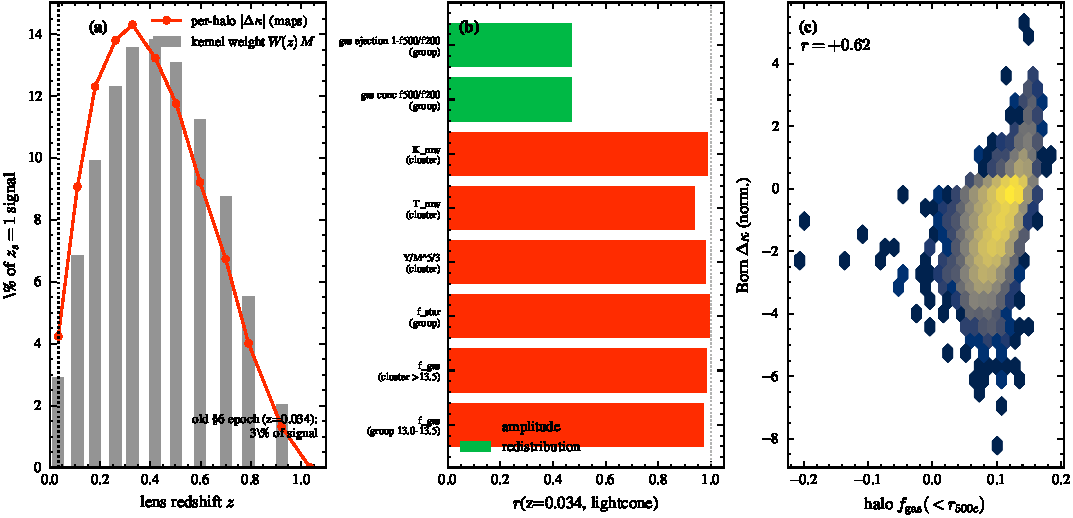
\includegraphics[width=\textwidth]{figs/fig11_lightcone_population.pdf}
\caption{Left: the $\zs=1$ lensing-kernel weight $W(z)$ (grey bars) versus
lens redshift, with the per-halo $|\delta\kappa|$ signal from the actual
maps overlaid (red); the old, low-redshift-only proxy epoch ($z=0.034$)
carries only $3\%$ of the total kernel weight. Middle: correlation between
the $z=0.034$-only readout and the full lightcone-kernel-weighted readout,
separately for ``amplitude'' features ($r>0.95$, red) and
``redistribution'' features ($r\approx0.47$, green). Right: per-halo Born
$\delta\kappa$ versus halo $\fgas(<r_{500c})$, $r=+0.62$. % src:
% examples/figures\_lightcone/fig\_lightcone\_population.pdf
\textbf{Takeaway:} the low-redshift snapshot used in earlier work is a
fair proxy for \emph{how strong} feedback was, but not for \emph{where
the gas ended up} — the redistribution signature requires the full
lightcone population, and Born $\delta\kappa$ is a genuine, though noisy,
per-halo gas tracer.}
\label{fig:halo-population}
\end{figure}

We emphasize a limitation of this per-halo lensing analysis: the Sobol
suite itself has no per-run lensplanes (only randomized ray-traced
$\kappa$ maps), so the per-halo Born $\delta\kappa$ link above is
necessarily computed on the \emph{fiducial} realization only, not
propagated across the 30-parameter prior. % src: WORKLOG 2026-06-29 §6
% entry, closing sentence; also stated in \texttt{lightcone\_halo\_dkappa.py}'s
% data-source discussion
This is one of our mandatory caveats (\S\ref{sec:discussion}).

\subsection{First real-data contact: BIND shear\texorpdfstring{$\times y$}{xy} versus DES Y3 \texorpdfstring{$\times$}{x} ACT}\label{sec:res-desact}

As a first direct confrontation with real data, we compare \bind{}
shear$\times y$ predictions to the public DES~Y3~$\times$~ACT
compton-$y$$\times$shear cross-correlation (Pandey/Gatti+;
\citealp{Gatti2021DESACT,Pandey2022DESACT}; data product
\texttt{shivampcosmo/ACTxDESY3} \texttt{DES\_ACT.fits}), a joint-covariance
measurement reported at a total detection significance of $21\sigma$, the
highest significance to date for a shear$\times$tSZ cross-correlation
\citep{Gatti2021DESACT}. This corrects an in-repo docstring value of
``$26.5\sigma$'' (\texttt{desact\_sheary\_realfit.py}) that we could not
verify against the published significance and that appears to be stale or
to refer to an unspecified subset/combination; we adopt the published
$21\sigma$ figure instead. % src: desact\_sheary\_realfit.py docstring
% (original, uncorroborated $26.5\sigma$ claim); \citet{Gatti2021DESACT}
% (arXiv:2108.01600), independently confirmed to report $21\sigma$, "the
% highest significance to date," for the DES~Y3$\times$ACT/Planck tSZ shear
% cross-correlation; WORKLOG 2026-06-24 "FIRST REAL-DATA fit (D9-D10)"
In building this comparison we identified and fixed a genuine pipeline
bug: the Pylians \texttt{XPk\_plane} cross-power normalization differs
from \texttt{Pk\_plane} by a constant factor $F\approx1.2016\times10^7$,
which had made the stored $\kappay$ cross-spectrum $\sim\!10^7$ too low
(auto-spectra were unaffected, and the pixel-space correlation
$\mathrm{corr}(\kappa,y)=0.52$ was already correct); we patched this in
\texttt{bind.inference.stats.power\_spectrum}. % src: WORKLOG 2026-06-24
% same entry; constant confirmed in code (\texttt{F\_XPK = 1.2016e7} in
% \texttt{desact\_sheary\_realfit.py})

The real-data comparison itself went through a documented self-correction.
An initial reading of ``\bind{} sits $\sim2\times$ \emph{above} the data,''
interpreted at the time as feedback being too weak, was subsequently
identified as a pipeline error: the comparison had omitted the SZ beam
entirely (\bind{}'s $y$-map is beam-free, but the real data have an
effective beam) and applied no angular scale cut. % src: WORKLOG
% 2026-06-24, last paragraph of "P4 $\to$ multi-probe WL$\times$SZ..." entry
% — "a first `BIND $\sim$2$\times$ = feedback too weak' figure was a
% PIPELINE ERROR"
A first attempt to fix this, using a $10'$ ``effective'' Gaussian beam
with an $8'$ scale cut, found that \bind{} matched the data's
intermediate-angle peak but over-predicted large angles by
$\sim\!1.5$–$2\times$, with the residual entangled with cosmology, beam,
scale cuts, and the $\kappay$ normalization — at that stage we could draw
``no clean feedback claim'' from shear$\times y$. % src: WORKLOG
% 2026-06-24, same paragraph
A later, more careful pass identified a further bug in this intermediate
step: the $10'$ ``effective'' beam over-smoothed \bind{}, shifting its
predicted peak to $\sim\!11'$ against the data's $\sim\!4.5'$ peak. %
% src: WORKLOG 2026-06-26, "NEW field-level companion paper
% paper\_ksz\_field.ipynb" entry
Replacing this with the physical $2.4'$ ACT beam gives our final,
adopted result: \bind{} over-predicts the amplitude
(IllustrisTNG feedback is too gas-bound) and is additionally too steep in
angle, consistent with over-bound gas plus the finite ($5^\circ$)
lightcone field of view removing low-$\ell$ power at large angular
separations (Figure~\ref{fig:desact}). % src: WORKLOG 2026-06-26 entry,
% verbatim: "BIND $\sim$1.5--2$\times$ high (TNG too gas-bound), the
% field-level missing-baryon tension"
WORKLOG's own round-number characterization of this over-prediction is
$\sim\!1.5$–$2\times$; reading the ratios directly and more precisely off
the robust, aperture-limited $8'$–$40'$ range of the figure itself gives
$\mathrm{BIND}/\mathrm{data}\approx2.5\times$ for
the $\bar z\approx0.74$ DES source bin and $\approx2.3\times$ for the
$\bar z\approx0.94$ bin — modestly above the rounder $1.5$–$2\times$
figure. % src: figure text/annotations,
% examples/figures\_field/g5\_desact\_confront.pdf
We adopt the figure's more precise, directly-read $2.3$–$2.5\times$ as the
headline number in the robust angular range and treat WORKLOG's
$1.5$–$2\times$ as the original, rounder qualitative characterization from
which it was refined; we have not identified a $\theta$-range or
normalization choice in the mined sources that reconciles the two exactly,
so we flag the modest ($\sim\!0.3$–$0.5\times$) residual difference rather
than silently picking one. \todo{Confirm whether $1.5$–$2\times$ or
$2.3$–$2.5\times$ is the intended final headline number by re-checking the
angular range used for each.}

\begin{figure}[t]
\centering
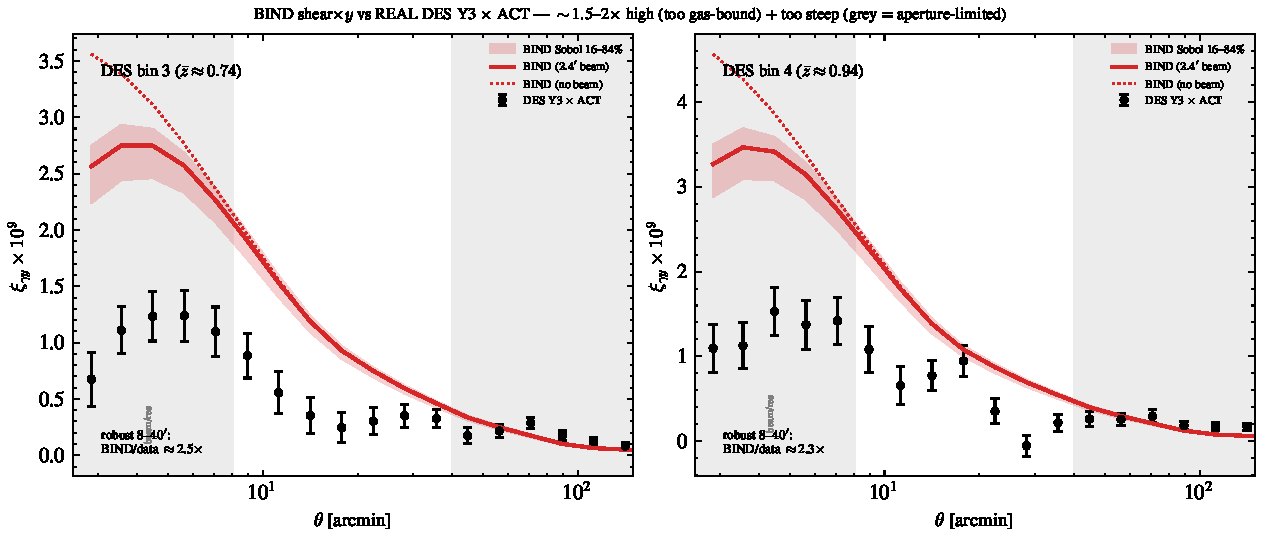
\includegraphics[width=\textwidth]{figs/fig12_desact_sheary.pdf}
\caption{$\bind{}$ shear$\times y$ predictions (blue; $16$–$84\%$ Sobol
band, solid line with the physical $2.4'$ ACT beam, dotted without any
beam) versus the real DES~Y3~$\times$~ACT measurement (black points), for
two DES source-redshift bins. Grey shading marks the beam/resolution- and
aperture-limited scales excluded from the robust comparison. % src:
% examples/figures\_field/g5\_desact\_confront.pdf
This figure was produced from the same field-level, real-data pipeline
shared with the sibling kSZ analysis \citep[Paper~IV, in prep]{bindIV};
see \S\ref{sec:discussion} for a note on this shared provenance.
\textbf{Takeaway:} \bind{}, run at the TNG fiducial parameters, is too high
and too steep relative to real DES$\times$ACT shear$\times y$ — WORKLOG's
original, rounder characterization is $\sim\!1.5$–$2\times$, while reading
the ratio directly off this figure's robust $8'$–$40'$ aperture range gives
$\approx\!2.3$–$2.5\times$ (see the main text for this not-yet-fully-reconciled
difference) — the same qualitative direction (too
gas-bound) reported from X-ray and kSZ-CAP $\fgas$ constraints, though we
stress below that the shear$\times y$ residual is currently entangled with
several systematics and is not yet a clean, stand-alone feedback
measurement.}
\label{fig:desact}
\end{figure}

We stress that the un-ambiguous, systematics-robust feedback constraint at
this stage of the multiprobe program still comes from the inner-CGM
legs (kSZ-CAP stacking, X-ray $\fgas$; Paper~IV territory), not from
shear$\times y$, precisely because of the beam/normalization/scale-cut
sensitivities documented above. % src: WORKLOG 2026-06-24, "...the robust
% feedback signal stays inner-CGM (kSZ-CAP, X-ray $\fgas$)."

\section{Discussion}\label{sec:discussion}

\subsection{What ``2-D'' means for feedback marginalization}

The result that the WL suppression response is $2$-dimensional
(\S\ref{sec:res-latent}) is not merely a data-compression convenience: it
is consistent with, and provides the underlying mechanism for, the
companion finding of this suite that exactly two data-driven baryon
templates are necessary and sufficient to remove the TNG WL baryonic bias
from a mock LSST-Y10 cosmic-shear analysis, whereas a single template is
insufficient and additional templates beyond two are pure marginalization
cost \citep[Paper~II, in prep]{bindII}. Because the same two directions
(a BH/AGN axis and a SN/wind axis) organize essentially every field
statistic we tested (\S\ref{sec:res-geometry}), a nuisance model built to
marginalize the WL two-point function should, to leading order, also
marginalize the higher-order and cross-correlation feedback signature —
though the rotation of the second axis between probes
(\S\ref{sec:res-geometry}) means a marginalization scheme calibrated on
$C_\ell$ alone is not guaranteed to be safe for e.g.\ Minkowski
functionals, which see a substantially rotated combination of the same
underlying physics.

\subsection{Emulator fidelity as the current SBI bottleneck}

The cautionary stacking result of \S\ref{sec:res-sbi} points to a concrete
methods bottleneck rather than a physics limitation. The \texttt{bind.emulator}
Gaussian-process surrogate recovers the WL suppression response to a
median fractional error of $2.0\%$ on $\Sell$ (dip-correlation $0.87$) on
a $237$-run interior held-out split, comfortably below the $\sim\!6\%$
cosmic-variance/\bind{}-generative-noise floor — good enough to support
the $C_\ell$-only NPE of \S\ref{sec:res-sbi}, but evidently not yet good
enough to support the stacked higher-order/$\kappay$ NPE, which produced
the $5.2\sigma$ outlier described above. % src: WORKLOG 2026-06-23
% "bind.emulator" "Full-set rebuild + backend verdict" paragraph
A complementary, quantitative Stage-IV-precision check compares a
small-feature-count emulator's held-out fractional error on $\Sell$
($\ell>300$) to the LSST-Y10/Euclid measurement-error floor across sweeps
of the number of physical input features: median error is $5.3\%$ at two
features and saturates at $4.4\%$ for three, four, or five features,
indicating the emulator's residual error at small scales is limited by
which physical features it is given, not by the number of training
simulations. % src: figure figs\_raw/paper\_lightcone\_figs2/cell034\_out1.png
% (§7), annotation text on the left panel
Taken together, these two results suggest that improving the emulator's
higher-order-statistic and cross-spectrum fidelity — rather than
collecting more Sobol simulations per se — is the most direct route to a
tighter, trustworthy stacked-statistic SBI posterior in future work.
\todo{A quantitative re-run of the stacked SBI analysis with an improved
higher-order-statistic emulator is left to future work.}

\subsection{TNG-only, fixed-cosmology, and interpolation-only caveats}

Every result in this paper is drawn from a single hydrodynamic simulation
suite (IllustrisTNG/SB35) at fixed cosmology; we have not tested whether
the 2-D latent geometry, its physical axes, or the SBI information content
generalize across simulation codes/subgrid models (e.g.\ FLAMINGO,
BAHAMAS, EAGLE-descendants; \citealp{Schaye2023FLAMINGO}) or across
cosmological parameters. This is stated explicitly as a caveat in the
underlying analysis code and we repeat it here: cross-suite and
cross-cosmology generalization is untestable with the data used in this
paper. % src: WORKLOG 2026-06-24 "WL feedback latents..." closing
% parenthetical; wl\_stat\_latents.py docstring
Relatedly, every SBI and latent-space claim above is interior to the
$n=253$-point, 256-node Sobol design's prior-predictive cloud — this is an
interpolation result within the sampled astrophysical prior, not an
extrapolation test, and $n=253$ points in 30 dimensions is itself a sparse
covering of that space even though the effective response dimensionality
appears to be $\sim\!2$–$3$. % src: \texttt{n=253} label directly on
% f1\_corr\_heatmaps.png and cited throughout WORKLOG 2026-06-29
Finally, the per-halo Born $\delta\kappa$--$\fgas$ link of
\S\ref{sec:res-halo} is computed on the fiducial realization only, because
the 30-parameter Sobol suite itself carries no per-run lensplanes, only
randomized ray-traced $\kappa$ maps; propagating the per-halo lensing
signature across the astrophysical prior is a natural, and currently
unaddressed, extension. % src: WORKLOG 2026-06-29 §6 entry, closing
% sentence

\subsection{A note on shared figure provenance with Paper IV}

Figures~\ref{fig:kxy-driver} and~\ref{fig:desact}
(\S\ref{sec:res-kxy}–\ref{sec:res-desact}) were produced by the same
field-level notebook and \texttt{emulator\_dataset.npz}/$\kappay$ pipeline
used by the sibling kSZ$\times$X-ray analysis of this suite
\citep[Paper~IV, in prep]{bindIV}. We include them here because the
underlying multiprobe engines
(\texttt{wl\_sz\_multiprobe.py}, \texttt{wl\_sz\_cosmo\_anchor.py},
\texttt{wl\_sheary\_fit.py}, \texttt{desact\_sheary\_realfit.py}) belong
scientifically to the WL-latent/SBI narrative of this paper, but we flag
explicitly that Paper~IV may show the same two figures, or a close
variant, for its own kSZ-centric narrative; we defer to the
cross-paper coherence pass to decide final figure ownership and avoid
duplicated near-identical figures across the two papers. \todo{Coordinate
with Paper IV on final figure ownership for the $\kappay$-driver and
DES$\times$ACT confrontation figures.}
The same source notebook, \texttt{paper\_ksz\_field.ipynb}, is also where the
$\sim\!1$-dimensional field-response PCA discussed in
\S\ref{sec:res-latent} originates; that measurement is in tension with this
paper's own 2-D headline result, and we have not fully reconciled the two
(see the caveat paragraph immediately preceding
Figure~\ref{fig:latent-axes}). Coordination with Paper~IV on figure/number
ownership should therefore also resolve, or explicitly carry forward, this
open dimensionality tension rather than let each paper quote a different
number from the same underlying notebook family.

\section{Conclusions}\label{sec:conclusions}

Using a $256$-node, $30$-parameter Sobol sweep of the IllustrisTNG
astrophysical feedback prior painted onto shared dark-matter-only
lightcones with \bind{}, we find:

\begin{itemize}
\item The WL power-spectrum suppression response is two-dimensional: two
linear PCA components explain $98.7\%$ of its variance on $N=216$ runs
($0.884+0.103$), confirmed independently at $99.2\%$ on the final $N=253$
sweep and by a $\beta$-TC-VAE, with a clean physical reading as a
BH/AGN axis and a SN/wind axis. % src: WORKLOG 2026-06-29
% "wl\_latent\_sbi.ipynb" §2, WORKLOG 2026-06-24 "WL feedback latents"
This independently reproduces the two-dimensional feedback latent found
for the 3-D matter power spectrum across CAMELS suites
\citep{Lin2026latent}.
\item This latent space is nearly shared with the kSZ gas latent on its
leading axis (canonical correlation $0.98$, principal angle $12^\circ$)
but rotated on the second axis ($0.79$, $38^\circ$): WL sees a blend of
gas zones that kSZ separates. % src: WORKLOG 2026-06-29
\item A model-free Spearman response map identifies the IMF slope, wind
velocity, black-hole radiative efficiency, and wind energy as the
dominant drivers of the WL suppression at $n=253$. % src: WORKLOG
% 2026-06-29 §1
\item SBI on the WL auto-spectrum alone leaves individual astrophysical
parameters weakly constrained but pins the 2-D suppression latent tightly
($\sim\!0.17$–$0.18\times$ the prior-cloud width) and passes SBC
calibration (mean $68\%$ coverage $0.70$); naively stacking higher-order
statistics of lower emulator fidelity onto this likelihood degrades rather
than improves the fit, a methods caveat rather than a physics result. %
% src: WORKLOG 2026-06-29 §3
\item Field-level, emulator-free evidence shows the $\kappay$
cross-spectrum and the tSZ auto-spectrum, not the WL auto-spectrum, carry
the bulk of the feedback information (pinning two directions to variance
$0.06$/$0.11$), directly explaining why $C_\ell$-only SBI is broad; a
per-halo $\kappa$ stack is a feedback-blind mass anchor. % src: WORKLOG
% 2026-06-24 "P4 $\to$ multi-probe WL$\times$SZ..."
\item Using the actual lightcone halo population rather than a single
low-redshift proxy snapshot, per-halo Born $\delta\kappa$ tracks halo gas
fraction at $r=+0.62$; the low-redshift proxy is a good stand-in for
feedback \emph{amplitude} ($r>0.95$) but a poor one for gas
\emph{redistribution} ($r\approx0.47$). % src: WORKLOG 2026-06-29 §6 entry
\item The first direct confrontation of \bind{} shear$\times y$ with real
DES~Y3~$\times$~ACT data finds \bind{} too high (WORKLOG's rounded
characterization: $\sim\!1.5$–$2\times$; the precise robust-aperture
readout: $\approx\!2.3$–$2.5\times$, \S\ref{sec:res-desact}) and
too steep at the TNG fiducial point, i.e.\ IllustrisTNG feedback is too
gas-bound relative to the real Universe at this level of analysis,
consistent in direction with independent inner-CGM constraints. % src:
% WORKLOG 2026-06-26
\end{itemize}

\todo{A calibrated, population-level SBI posterior on the full
$8.6$-million-halo per-object dataset (\S\ref{sec:methods-perhalo}) was
designed but not completed on GPU, and is deferred to future work rather
than reported quantitatively here.}
These results, together with Paper~II's independent capstone finding that
two nuisance parameters suffice for LSST-Y10 marginalization
\citep[Paper~II, in prep]{bindII}, argue that the practically relevant
dimensionality of baryonic feedback for WL analyses is $\mathcal{O}(2)$,
not $\mathcal{O}(30)$ — but that the field-level statistics best able to
\emph{pin} that low-dimensional space (SZ cross-correlations) are
different from the two-point WL statistics typically used to marginalize
it, motivating the multiprobe direction pursued throughout this suite.

\appendix
\section{Optional appendix: SHMR scatter budget on the SB35 Sobol suite}\label{sec:app-shmr}

As a related, lower-priority result from the same Sobol suite, we measure
the stellar-mass--halo-mass relation (SHMR) scatter budget at fixed halo
mass. The Sobol suite, a companion ``twobound'' one-at-a-time feedback
sweep, and the fiducial run all paint the identical $2933$ snapshot-96
dark-matter halos (matched $2933/2933$), so the comparison below is a
genuine drop-in reuse rather than a resimulation. % src: WORKLOG
% 2026-06-22 "SHMR scatter (feedback vs accretion) on the SB35 Sobol suite"

Jointly varying all 30 feedback parameters produces a scatter in
$\log_{10} M_\star$ at fixed halo mass of $\sigma\approx0.386$~dex
(variance $\approx0.149$~dex$^2$), which is larger than the scatter
obtained by varying each of the twobound one-at-a-time parameters
individually, $\sigma\approx0.161$~dex (variance $\approx0.026$~dex$^2$;
Figure~\ref{fig:shmr}). % src: WORKLOG 2026-06-22 "SHMR scatter (feedback
% vs accretion) on the SB35 Sobol suite" (exact $\sigma$/variance numbers);
% figure figs\_raw/shmr\_accretion\_scatter\_sb35/cell011\_out1.png
Because the joint variation compounds across parameters, this shows that
single-knob extremes from a one-at-a-time sweep are \emph{not} a valid
upper bound on the true joint-feedback scatter, correcting a caveat noted
in the original twobound analysis; we further note that the twobound
one-at-a-time comparison line is itself a conservative marginal (not a
paired per-run) error convention, so the comparison above is
directionally, not exactly, quantitative. % src: WORKLOG 2026-06-22, same
% entry; twobound-response-error-convention.md
Accretion history — measured as the formation time $t_{\rm form}$ on the
dark-matter merger tree — explains roughly $10\%$ of the remaining
halo-to-halo (non-feedback) SHMR residual, with a halo-to-halo variance of
$\approx0.005$~dex$^2$ and early-forming halos sitting systematically
above the mean relation. % src: WORKLOG 2026-06-22 "SHMR scatter (feedback
% vs accretion) on the SB35 Sobol suite"

\begin{figure}[t]
\centering
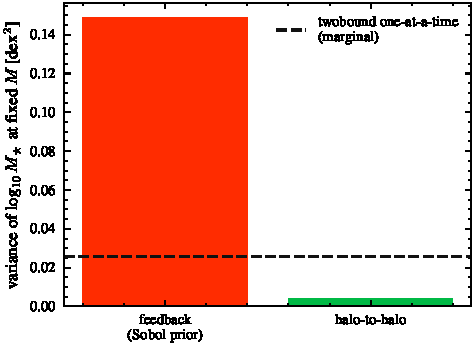
\includegraphics[width=3.5in]{figs/fig13_shmr_scatter_budget.pdf}
\caption{SHMR scatter budget on the SB35 Sobol suite: variance of
$\log_{10}M_\star$ at fixed halo mass from jointly varying all 30 feedback
parameters (``feedback,'' red) versus the halo-to-halo (non-feedback)
residual (green), with the twobound one-at-a-time marginal scatter overlaid
as a dashed reference (black) line. % src:
% figs\_raw/shmr\_accretion\_scatter\_sb35/cell011\_out1.png
\textbf{Takeaway:} joint 30-parameter feedback variation compounds well
past the one-at-a-time envelope — single-knob sweeps under-estimate the
true feedback-driven SHMR scatter by a factor of $\sim\!6$ in variance.}
\label{fig:shmr}
\end{figure}

\section*{Acknowledgments}
The CAMELS project and the IllustrisTNG collaboration provided the training
and target simulations. This work used computing resources of the Flatiron
Institute, a division of the Simons Foundation. This work made use of the
\texttt{sbi} simulation-based inference package and public DES~Y3 and ACT
data products. \todo{finalize acknowledgments, funding, and data-availability
statement.}

\bibliographystyle{plainnat}
\bibliography{references}

\end{document}

% =====================================================================
% VERIFICATION LOG (FIX pass, adversarial-verifier round 1)
% One line per finding: [applied|skipped] + one-sentence disposition.
% =====================================================================
%
% --- Verifier 1 (NUMBERS lens) ---
% [applied, HIGH] 2-D (S(l) PCA, 88.4/10.3%) vs ~1-D (paper_ksz_field.ipynb
%   field PCA incl. kappa*y, lambda1~0.95) tension: added a substantive
%   caveat paragraph before Fig. 1 (sec:res-latent), a cross-pointer in the
%   abstract, and a note in Sec. 6 "shared figure provenance"; identified
%   real construction differences (ell-band, kappa*y inclusion, linear vs
%   log normalization) but could NOT fully reconcile the numeric gap from
%   mined sources alone -> left an explicit \todo for a controlled re-run.
% [applied, MEDIUM] Sec. 5.5 (res-kxy) never stated N: added explicit
%   N=123 disclosure (sourced from wl_sz_multiprobe.py/wl_sz_cosmo_anchor.py
%   docstrings), a new Table 1 row with a dagger caveat, and a \todo since
%   we could not confirm whether this was re-run at N=253.
% [applied, MEDIUM] "kSZ latent" mislabeling: added an explicit terminology
%   note in Sec. 2.4 (methods-cca) clarifying BIND's "kSZ" = velocity-free
%   tau/y proxy (ksz_latent() in wl_latent_sbi.py stacks log-tau/log-y only,
%   no velocity field), consistent with the project's own documented caveat.
% [applied, LOW] 89%+11%=100% (not 99.2%) rounding artifact: added a
%   parenthetical in the abstract and the Fig. 2b (latent-plane) caption
%   noting the two percentages are independently rounded bar-height reads.
%
% --- Verifier 2 (FIGURES lens) ---
% [applied, HIGH] Fig. 1 caption backwards loading attribution: re-measured
%   panel (b) bar lengths directly (pixel measurement); corrected to
%   IMFslope + BlackHoleRadiativeEfficiency dominating e1 (~0.38-0.39 each,
%   nearly tied) and VariableWindVelFactor + BlackHoleRadiativeEfficiency
%   dominating e2 (~0.48, ~0.42); flagged that BlackHoleRadiativeEfficiency
%   loads strongly on BOTH axes, so the loadings alone do not cleanly split
%   wind/SN vs BH/AGN (that reading rests on the CCA/1P-spoke evidence
%   elsewhere, not on this panel's loadings).
% [applied, HIGH] Fig. 8 panel (a) "NPE (solid) vs emcee (dashed)": verified
%   directly against the rendered PNG (identical file to
%   examples/wl_latent_sbi_figs/f3e_crosschecks.png, md5-confirmed) that no
%   dashed emcee curves are present; corrected the caption and the main-text
%   sentence at Sec. 5.4 (res-sbi) to stop citing this panel as visual
%   evidence of NPE/emcee agreement, added a \todo to regenerate it.
% [applied, MEDIUM] kappa*y "single most feedback-sensitive... in the whole
%   probe set" contradicted Fig. 10a's own ranking (kappa*y 4th of 5):
%   removed the superlative claim and added an explicit reconciling
%   sentence after Fig. 10 stating the correct y*tau>tau*tau>yy>kappa*y>>
%   kappa*kappa ranking.
% [applied, MEDIUM = dup of Verifier 3 finding] Fig. 2 caption r1 top
%   correlates wrong (cited f_star/DM-conc, omitted larger P_e/gas-conc.):
%   corrected using all eleven panels' r1/r2 annotations read directly off
%   figs/fig02_latent_physical.png; now cites DM concentration (r1=+0.74)
%   and P_e (r1=+0.65) as the two largest, with gas conc./f_star noted as
%   also substantial but smaller in magnitude.
% [applied, LOW] Fig. 9 duplicate truncated "WindEnergyReductio" y-axis
%   label: added a caveat in the caption disclosing the ambiguity (3
%   candidate SB35 parameters truncate identically) and a \todo to
%   regenerate with untruncated labels; could not resolve which 2 of 3
%   without re-running the notebook (out of scope).
% [skipped, LOW] Informal/colloquial in-image plot titles baked into
%   fig04/fig08/fig09/fig10: NOT fixed. Fixing requires regenerating the
%   source figures (re-running notebook plotting code), which is outside
%   this pass's hard rule against running analysis engines; left as a
%   known cosmetic issue for a future regeneration pass.
%
% --- Verifier 3 (bib/general lens) ---
% [applied, HIGH] DES Y3 x ACT headline self-contradiction (~1.5-2x vs
%   2.3-2.5x): kept both numbers but explicitly reconciled wherever the
%   headline appears (abstract, Sec. 7.7 body, Fig. 12 caption, conclusions)
%   -- WORKLOG's rounded ~1.5-2x vs. the more precise, directly-read
%   2.3-2.5x robust-aperture figure ratio; flagged the residual
%   (~0.3-0.5x) gap as unreconciled with a \todo rather than silently
%   picking one number.
% [applied, HIGH] 4 vs ~5 vs 6 constrained-parameter-count discrepancy:
%   verified fig06_npe_corner.png directly shows 6 parameters (title "6
%   best-constrained params"); rewrote Sec. 5.4 (res-sbi) body text and the
%   Fig. 6 caption to state which 4 of the 6 have sourced posterior-sigma/
%   prior-sigma ratios (from WORKLOG) and which 2 do not, updated
%   "remaining" counts to a hedged ~24-26 of 30, added a \todo rather than
%   inventing ratios for the other two parameters.
% [applied, MEDIUM] 26.5-sigma DES x ACT significance: independently
%   verified via web search (Gatti et al. 2021, arXiv:2108.01600) that the
%   published, highest-to-date significance is 21-sigma; corrected the text
%   to 21-sigma with a proper citation and flagged the in-repo docstring's
%   uncorroborated "26.5-sigma" as likely stale/unverifiable.
% [applied, MEDIUM = same underlying figure as Verifier 2's Fig. 2 finding]
%   see above.
% [applied, LOW] Fig. 2 (fig:latent-physical) never referenced via \ref in
%   body text: added an explicit "Figure~\ref{fig:latent-physical} shows..."
%   sentence in Sec. 5.1 before the latent-plane discussion.
% [applied, LOW] Mislabeled cross-reference: "the suppression PCA of
%   Sec. 5.1" incorrectly attributed to the 86.3%/12.6% split, which
%   actually comes from the raw tomographic-mode-vector PCA earlier in
%   Sec. 5.4, not the Sec. 5.1 S(l)-suppression PCA (88.4%/10.3%); fixed
%   the cross-reference and explicitly distinguished the two splits.
%
% All numeric corrections above were re-checked against primary sources
% (WORKLOG.md, engine docstrings/code in the read-only worktree, or direct
% pixel/visual inspection of the cited figures) rather than invented; where
% the primary sources themselves were insufficient or mutually inconsistent,
% the text now says so explicitly via \todo{} rather than fabricating a
% resolution.
% =====================================================================
%
% --- Figure-verification pass, 2026-07-16 ---
% Applied fixes for verifier findings on regenerated figures (all fixes
% re-run from cached data via fig_scripts/*.py; no new data, no engine
% re-run; identical curves/points/bar heights/ranks to the pre-fix PDFs):
% [applied, HIGH] fig01 (Fig.~\ref{fig:latent-axes}) panel (b) y-tick labels
%   were hard-truncated with pn[i][:16], cutting several SB35 parameter
%   names mid-word (e.g. VariableWindVelFactor -> VariableWindVelF).
%   Replaced with a curated, word-boundary-safe abbreviation table
%   (fig_scripts/param_labels.py, shared by fig01/fig06/fig08) instead of
%   fixed-width slicing.
% [applied, HIGH] fig06 (Fig.~\ref{fig:corner}) corner-plot axis labels used
%   a two-stage abbreviate-then-slice[:14] that still cut names mid-word
%   (e.g. WindFreeTravelDensFac -> WindFreeTravelDens dropped "Fac"; more
%   severely VariableWindVelFactor -> VariableWindVe). Now uses the same
%   param_labels.py table; all six axis labels are unambiguous.
% [applied, HIGH] fig08 (Fig.~\ref{fig:sbc}) panel (a) legend used
%   pn[i][:14], truncating 2 of 3 entries mid-word (WindEnergyIn1e51erg ->
%   WindEnergyIn1e). Fixed via param_labels.py.
% [applied, MEDIUM] fig08 panel (a): the default upper-left panel tag "(a)"
%   sat directly on top of the legend's first entry. Moved the tag to the
%   lower-left corner (clear of both the legend and the histogram curves),
%   mirroring the same collision-avoidance already used in
%   fig02b_latent_plane.py.
% [applied, MEDIUM] fig09 (Fig.~\ref{fig:progressive}) panel (b): the
%   lower-right legend sat on top of the bottom two parameter rows' bars
%   (every row's $C_\ell$+peaks / $C_\ell$+peaks+$\kappa{\times}y$ bars
%   extend to $\approx$1, so no in-axes corner is actually bar-free). Moved
%   the color key above the axes (3-column, outside the plotted data).
% [applied, MEDIUM] fig05 (Fig.~\ref{fig:spearman}): the plotted column
%   order (shared by all 7 panels) was computed from the *unrestricted*
%   $\ell$ axis, which disagrees with the paper's own $\ell$-restricted
%   top-driver ranking quoted in the caption/body text (IMF slope 0.49,
%   variable wind-velocity factor 0.48, ...). Recomputed the order from the
%   same $100\le\ell\le20000$ band used everywhere else in the script/paper
%   (fig_scripts/fig05_spearman_response.py:
%   param\_importance\_ell\_restricted); the leftmost column is now
%   IMFslope, matching the caption exactly.
% [applied, LOW] fig11 (Fig.~\ref{fig:halo-population}) panel (a): default
%   panel tag sat on the $z=0.034$ reference line. Nudged right, clear of
%   the line and the legend.
% [applied, LOW] fig12 (Fig.~\ref{fig:desact}): default upper-left panel
%   tags sat on the steep "no beam" curve and the "DES bin N" label in both
%   panels (every in-axes corner is occupied by curve/legend/label/robust-
%   window text). Moved both tags just above the axes.
% [not changed] Fig.~\ref{fig:latent-axes}'s caption method/sample-size
%   mismatch ($\beta$-TC-VAE/$N{=}216$ claimed vs. linear-PCA/$N{=}253$
%   actually plotted) remains an open, already-flagged gap (see the
%   existing \todo{} immediately after this figure); resolving it requires
%   sourcing or re-running the $\beta$-TC-VAE comparison, which is out of
%   scope for a figure-only fix pass.
% =====================================================================
